\documentclass[conference]{IEEEtran}

\usepackage{cite}
\usepackage{amsmath,amssymb,amsfonts}
\usepackage{algorithmic}
\usepackage{textcomp}
\usepackage{xcolor}
\usepackage{float}
\usepackage{multirow}
\usepackage{textcomp}

% *** GRAPHICS RELATED PACKAGES ***
\usepackage[pdftex]{graphicx}
\graphicspath{{./figures/}}
\DeclareGraphicsExtensions{.png}

% *** FOOTNOTES PACKAGE ***
\usepackage[bottom]{footmisc}


% References package
\usepackage[unicode=false,psdextra]{hyperref}

% Floating objects, captions and references
\usepackage{flafter}
\usepackage[noabbrev,nameinlink,capitalise]{cleveref}

\def\BibTeX{{\rm B\kern-.05em{\sc i\kern-.025em b}\kern-.08em
    T\kern-.1667em\lower.7ex\hbox{E}\kern-.125emX}}

\begin{document}

\title{Reddit classification}

\author{\IEEEauthorblockN{Pedro Escaleira}
\IEEEauthorblockA{Departamento de Electrónica\\ Telecomunicações e Informática\\
\textit{Universidade de Aveiro}\\
Aveiro, Portugal \\
escaleira@ua.pt}
\and
\IEEEauthorblockN{Rafael Simões}
\IEEEauthorblockA{Departamento de Electrónica\\ Telecomunicações e Informática\\
\textit{Universidade de Aveiro}\\
Aveiro, Portugal \\
rafaeljsimoes@ua.pt}
}

\maketitle

\begin{abstract}
Aprendizagem Automática é uma área das ciências da computação com cada vez mais destaque nos dias que correm. Desde a sua utilização em campos como a saúde, sistemas bancários, \textit{self driving cars}, nas aplicações de telemóvel do utilizador comum, entre outros, não é surpresa para ninguém que se tornou uma realidade sem a qual a sociedade em que vivemos seria muito diferente do que é hoje. \\
Neste relatório, iremos descrever a utilização de alguns dos algoritmos mais conhecidos e usados nesta área e o seu comportamento perante diferentes situações, usando para isso um \textit{dataset} de \textit{posts} criados na rede social \textit{Reddit}.

\end{abstract}

\section{Introdução}
Este trabalho, proposto pela professora Petia Georgieva, do Departamento de Electrónica Telecomunicações e Informática da Universidade de Aveiro, teve o intuito de consolidar e instigar a utilização e pesquisa dos conceitos apresentados na disciplina de Tópicos de Aprendizagem Automática.
Desta forma, estudamos o comportamento dos algoritmos \textbf{Redes Neuronais}, redes de \textbf{\textit{bayes}} e \textbf{Regressão Logística} no âmbito de um trabalho de \textit{text classification}, mais especificamente classificação de textos em \textit{sub-reddits}. 

A razão de termos escolhido este tema foi que ia de encontro a uma das \textit{features} que o projecto de informática dos dois autores possuía: analisar \textit{tweets} e obter qual o tema principal que era discutido nos mesmos. Para mais informações sobre este projecto é favor consultar a página \cite{informatics_project}.

Além da implementação e estudo dos algoritmos enumerados anteriormente, foi também feita a implementação e estudo aprofundado de pré-processamento e \textit{feature extraction} de texto.

\section{Ferramentas usadas}
Este projecto foi executado usando-se \textit{Python} como linguagem de referência. Contudo, para facilitar o nosso trabalho, usamos algumas bibliotecas \textit{open source}:
\begin{itemize}
\item \textit{Pandas}: usado para ler os dados dos \textit{datasets} originalmente em \textit{csv} para matrizes de \textit{numpy}.
\item \textit{NumPy}: usado para fazer cálculos matriciais mais facilmente.
\item \textit{Matplotlib}: usado para criação facilitada de gráficos e figuras.
\item \textit{scikit-learn}: usado para estudar alguns dos algoritmos de aprendizagem automática descritos neste relatório.
\item \textit{Keras} e \textit{TensorFlow}: usados para estudar alguns dos algoritmos de aprendizagem automática descritos neste relatório.
\item \textit{Pickle}: usado para armazenar e carregar os modelos treinados em ficheiros binários.
\end{itemize}

\section{Dados}

\subsection{Dados originais}
Os dados usados neste estudo foram obtidos e proporcionados pela \textit{Evoluation AI} \footnote{Os dados podem ser encontrados em: \url{https://www.kaggle.com/mswarbrickjones/reddit-selfposts}}. Estes consistem em \textit{self-posts} feitos no \textit{Reddit} entre 2016/06/01 e 2018/06/01 (2 anos). De forma a garantir alguma qualidade, os dados foram submetidos a filtragem por parte da \textit{Evoluation AI}:
\begin{itemize}
    \item \textit{Posts} submetidas noutra língua que não o inglês.
    \item \textit{Posts} submetidos por moderadores ou \textit{admins} do \textit{Reddit}.
    \item \textit{Posts} cujo \textit{body text} possui-se menos do que 256 ou mais do que 4096 caracteres.
    \item \textit{Posts} duplicados.
\end{itemize}

Desta maneira, o \textit{dataset} final é constituído por \textit{posts} de 1013 classes, sendo que cada uma possui 1000 \textit{posts}. Mais informações sobre o tratamento ao qual os dados foram submetidos ou sobre algum estudo feito sobre eles podem ser encontradas em \cite{data_paper}.

\subsection{Pré-processamento dos dados}
\label{subsub:data_pre_processing}

Sabendo que este trabalho se trata de um problema de \textit{text classification}, é inevitável que exista algum processamento dos dados de entrada (textos), já que a maioria dos modelos existentes não são compatíveis com entradas não numéricas. Para além de questões de conveniência, nesta etapa também é implementado um mecanismo de escolha de \textit{features}.

Para uma fácil compreensão dos mecanismos usados nesta etapa, a explicação vai ser feita de uma forma enumerada:
\begin{enumerate}
\item \textbf{Conversão de texto para \textit{tokens}}: Nesta fase os textos presentes no \textit{dataset} são transformados numa lista de \textit{tokens}:
\begin{itemize}
\item Divisão do texto numa lista de \textit{tokens}. Ex: word\textunderscore{tokenize}("At eight o'clock on Thursday morning.") = ['At', 'eight', "o'clock", 'on', 'Thursday', 'morning', '.'].
\item Todos os \textit{tokens} são convertidos para letra minúscula.
\item Pontuação é removida.
\item É realizado o processo de lematização nos verbos presentes. Ex: inflected: inflect, ate: eat.
\item São retirados os \textit{tokens} que estão incluídos no conjunto de \textit{stop words} inglesas.

\bigbreak
Supondo o seguinte cenário, em que se pretende converter o texto \textit{"Lemmatisation (or lemmatization) in linguistics is the process of grouping together the inflected forms of a word"} para uma lista de \textit{tokens} o \textit{output} esperado seria: ['lemmatisation', 'lemmatization', 'linguistics', 'process', 'group', 'together', 'inflect', 'form', 'word']
\end{itemize}

\bigbreak
\item \textbf{Conversão da lista de \textit{tokens} para uma matriz de \textit{TF-IDF features}}.
Apesar da transformação anterior em \textit{tokens}, é necessário uma nova etapa para conseguir extrair \textit{features} dos textos disponibilizados, para que estes sejam usados à posteriori no modelo de \textit{Machine Learning}. Para isso foi usado o algoritmo \textit{\textbf{TF*IDF}}, que é uma técnica de extracção de informação que pesa a frequência de um termo (\textbf{\textit{TF}}) i.e, o número de vezes que o termo aparece, e a frequência inversa de documento (\textbf{\textit{IDF}}) i.e, uma pontuação que define o quão importante é um termo relativamente ao \textit{corpus} total. O produto das pontuações \textbf{\textit{TF}} e \textbf{\textit{IDF}} de um termo é chamado de peso \textbf{\textit{TF*IDF}}. A raridade do termo cresce com o aumento da pontuação \textbf{\textit{TF*IDF}} do respectivo termo.

Para mais detalhes, é favor consultar \cite{TF_IDF_algorithm}.

Apenas de referir que nesta etapa foram consideradas todos os uni-gramas e bigramas. Após o processo estar completo este algoritmo retorna um conjunto de termos (palavras) com o respectivo valor \textbf{\textit{TF*IDF}} mapeado. Este conjunto de palavras define o vocabulário do nosso \textit{corpus}. 

\bigbreak
\item \textbf{Diminuição do vocabulário proveniente do algoritmo \textit{TF*IDF}}

O conjunto de palavras definido anteriormente reflecte a quantidade de \textit{features} de entrada para o nosso modelo, sendo que, como é expectável, este pode possuir dimensões elevadas. Devido a este facto, é essencial reduzir o numero de \textit{features} (numero de termos do vocabulário), para que os processos de treino sejam optimizados e para cumprir limites de \textit{hardware}. Apesar de aparentar que podemos retirar informação importante do nosso \textit{corpus}, a diminuição do vocabulário torna-se pouco influente se removermos os termos com valor baixo de \textbf{\textit{TF*IDF}} (termos que não transmitem informação útil sobre o \textit{corpus}).

Ordenando os termos de vocabulário por ordem decrescente do valor de \textbf{\textit{TF*IDF}}, obtemos um gráfico como o apresentado na figura \ref{diagram:data_n_knee}. Como se pode observar, este possui uma forma exponencial, sendo que os valores mais à esquerda (com maior valor de \textbf{\textit{TF*IDF}}) representam as palavras mais importantes no \textit{corpus}, logo o que nos interessa para o nosso vocabulário são as palavras mais importantes. Aqui reforça-se a ideia da necessidade de segmentar o vocabulário, pois este atinge dimensões na ordem dos milhões.

\begin{figure}[t]
\begin{center}
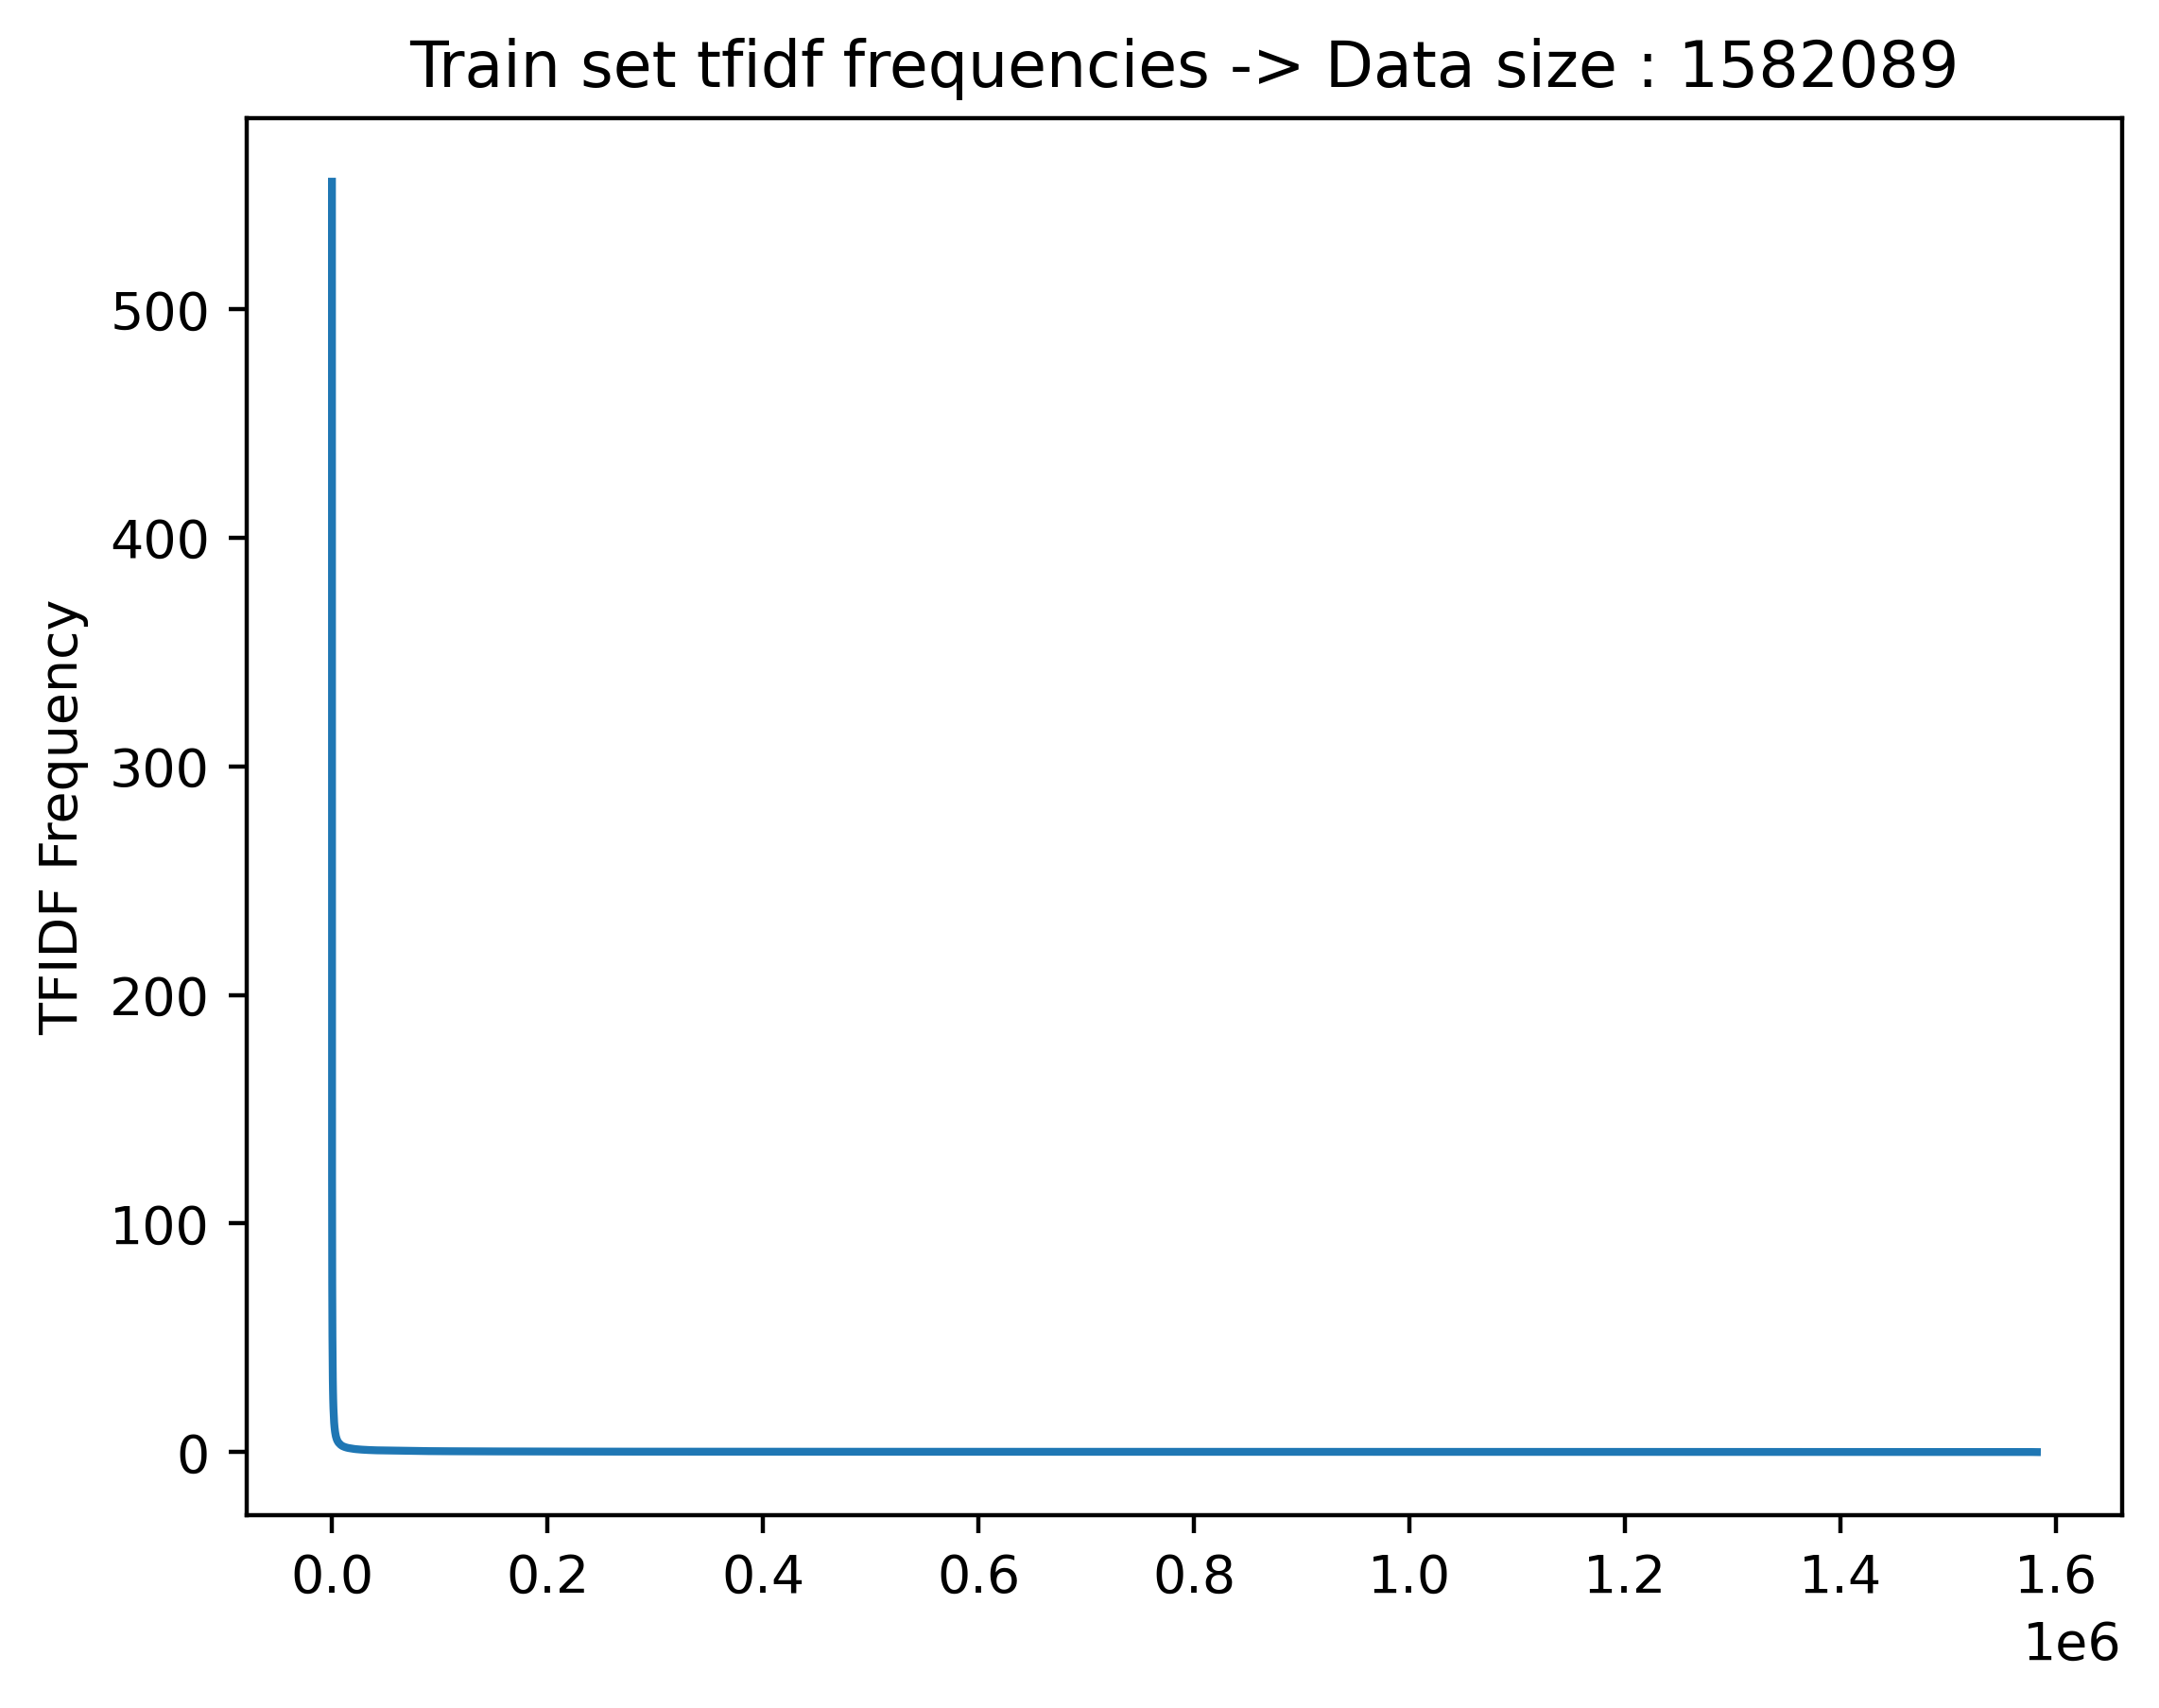
\includegraphics[width=0.5\textwidth,keepaspectratio]{figures/data_n_knee.png}
\caption{Frequências TF*IDF do corpus ordenados de forma decrescente }
\label{diagram:data_n_knee}
\centering
\end{center}
\end{figure}

Para conseguirmos segmentar os termos do vocabulário tendo em conta a forma de exponencial que este apresenta, foi usado o algoritmo \textit{Kneedle} \cite{Kneedle}, que tem como objectivo seleccionar o ponto onde o vocabulário deve ser cortado, sendo o ponto ideal o "joelho" (\textit{knee}) do gráfico. Basicamente o algoritmo escolhe o ponto ideal que divide os termos importantes dos não importantes.

Na figura \ref{diagram:data_knee}, podemos observar o \textit{knee\textunderscore{point}} que o algoritmo seleccionou, 7299. Isto implica uma redução de 99\% no tamanho do vocabulário inicial. 

\begin{figure}[t]
\begin{center}
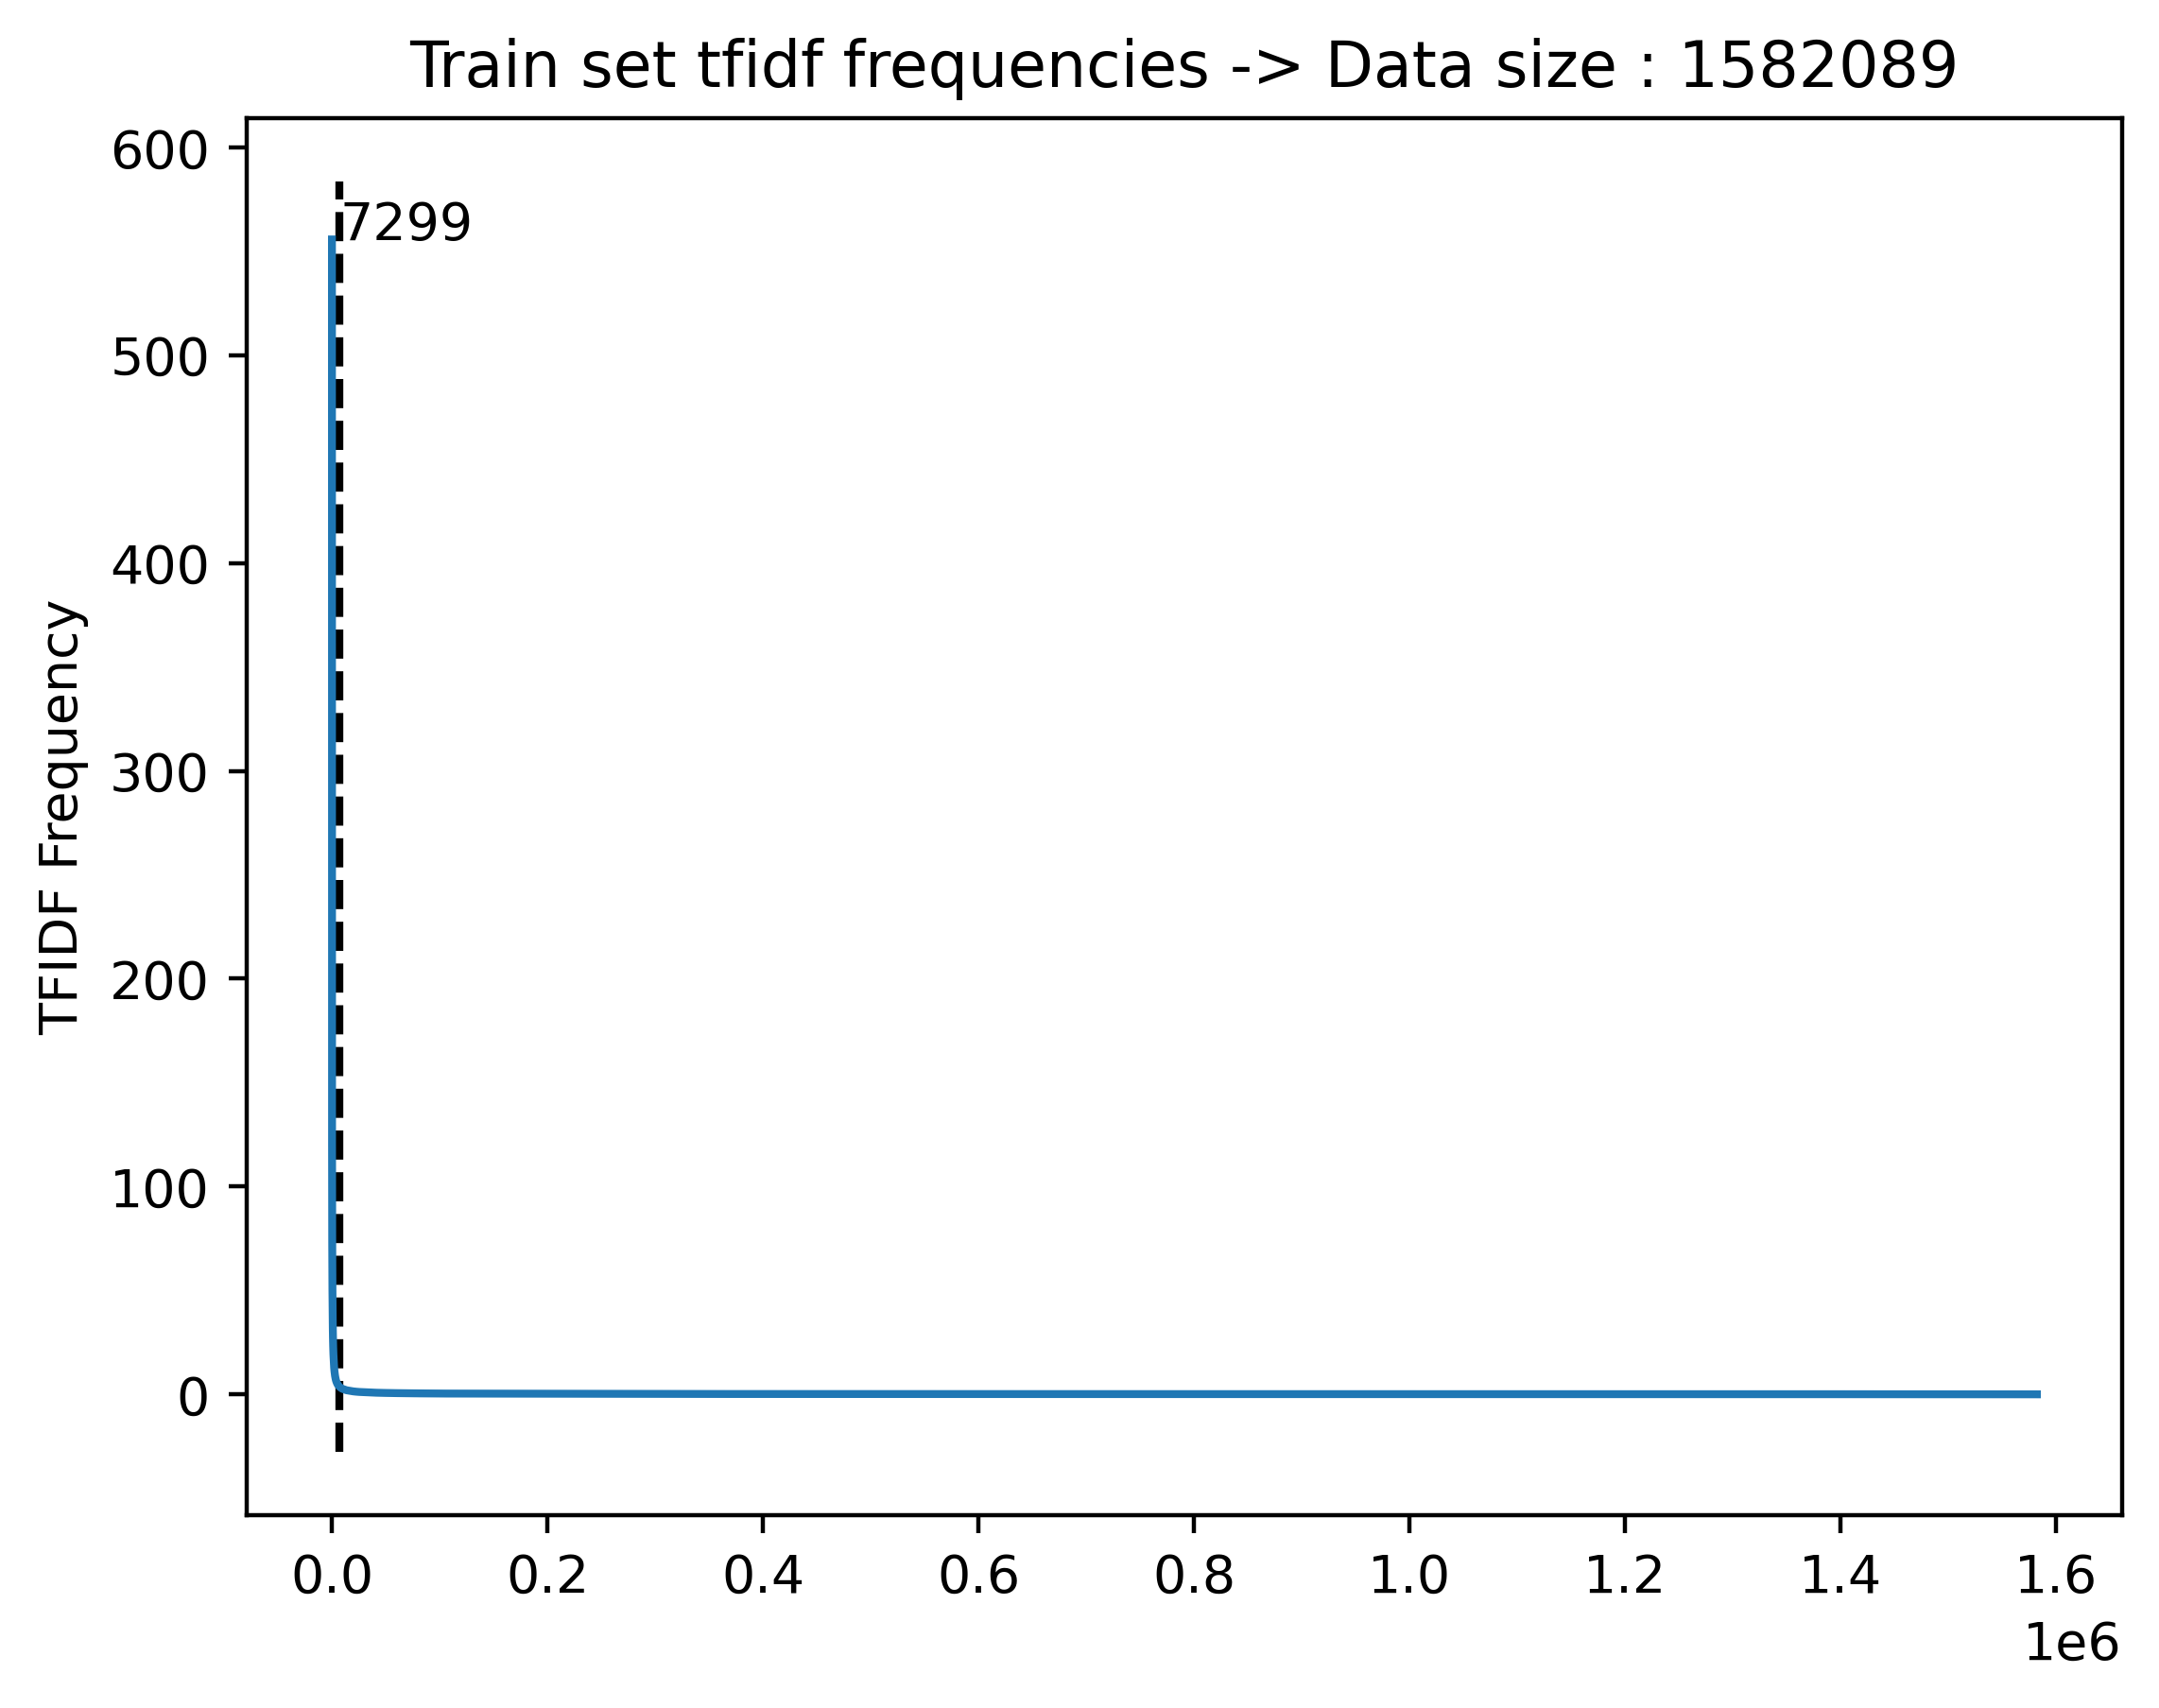
\includegraphics[width=0.5\textwidth,keepaspectratio]{figures/data_knee.png}
\caption{Frequências TF*IDF do corpus ordenados de forma decrescente com o \textit{knee\textunderscore{point}}}
\label{diagram:data_knee}
\centering
\end{center}
\end{figure}

Apesar da redução ser bastante significativa, 7299 termos de vocabulário continua a ser um número elevado de \textit{features}, sendo que para isso uma nova segmentação é realizada com o novo vocabulário reduzido. Como demonstrado na figura \ref{diagram:data_second_knee},  o novo vocabulário continua com a forma de exponencial. Posto isto, este processo é realizado até o algoritmo não conseguir encontrar o \textit{knee point} - este processo pode ser visualizado no gráfico \ref{diagram:data_all_knee}.

\begin{figure}[t]
\begin{center}
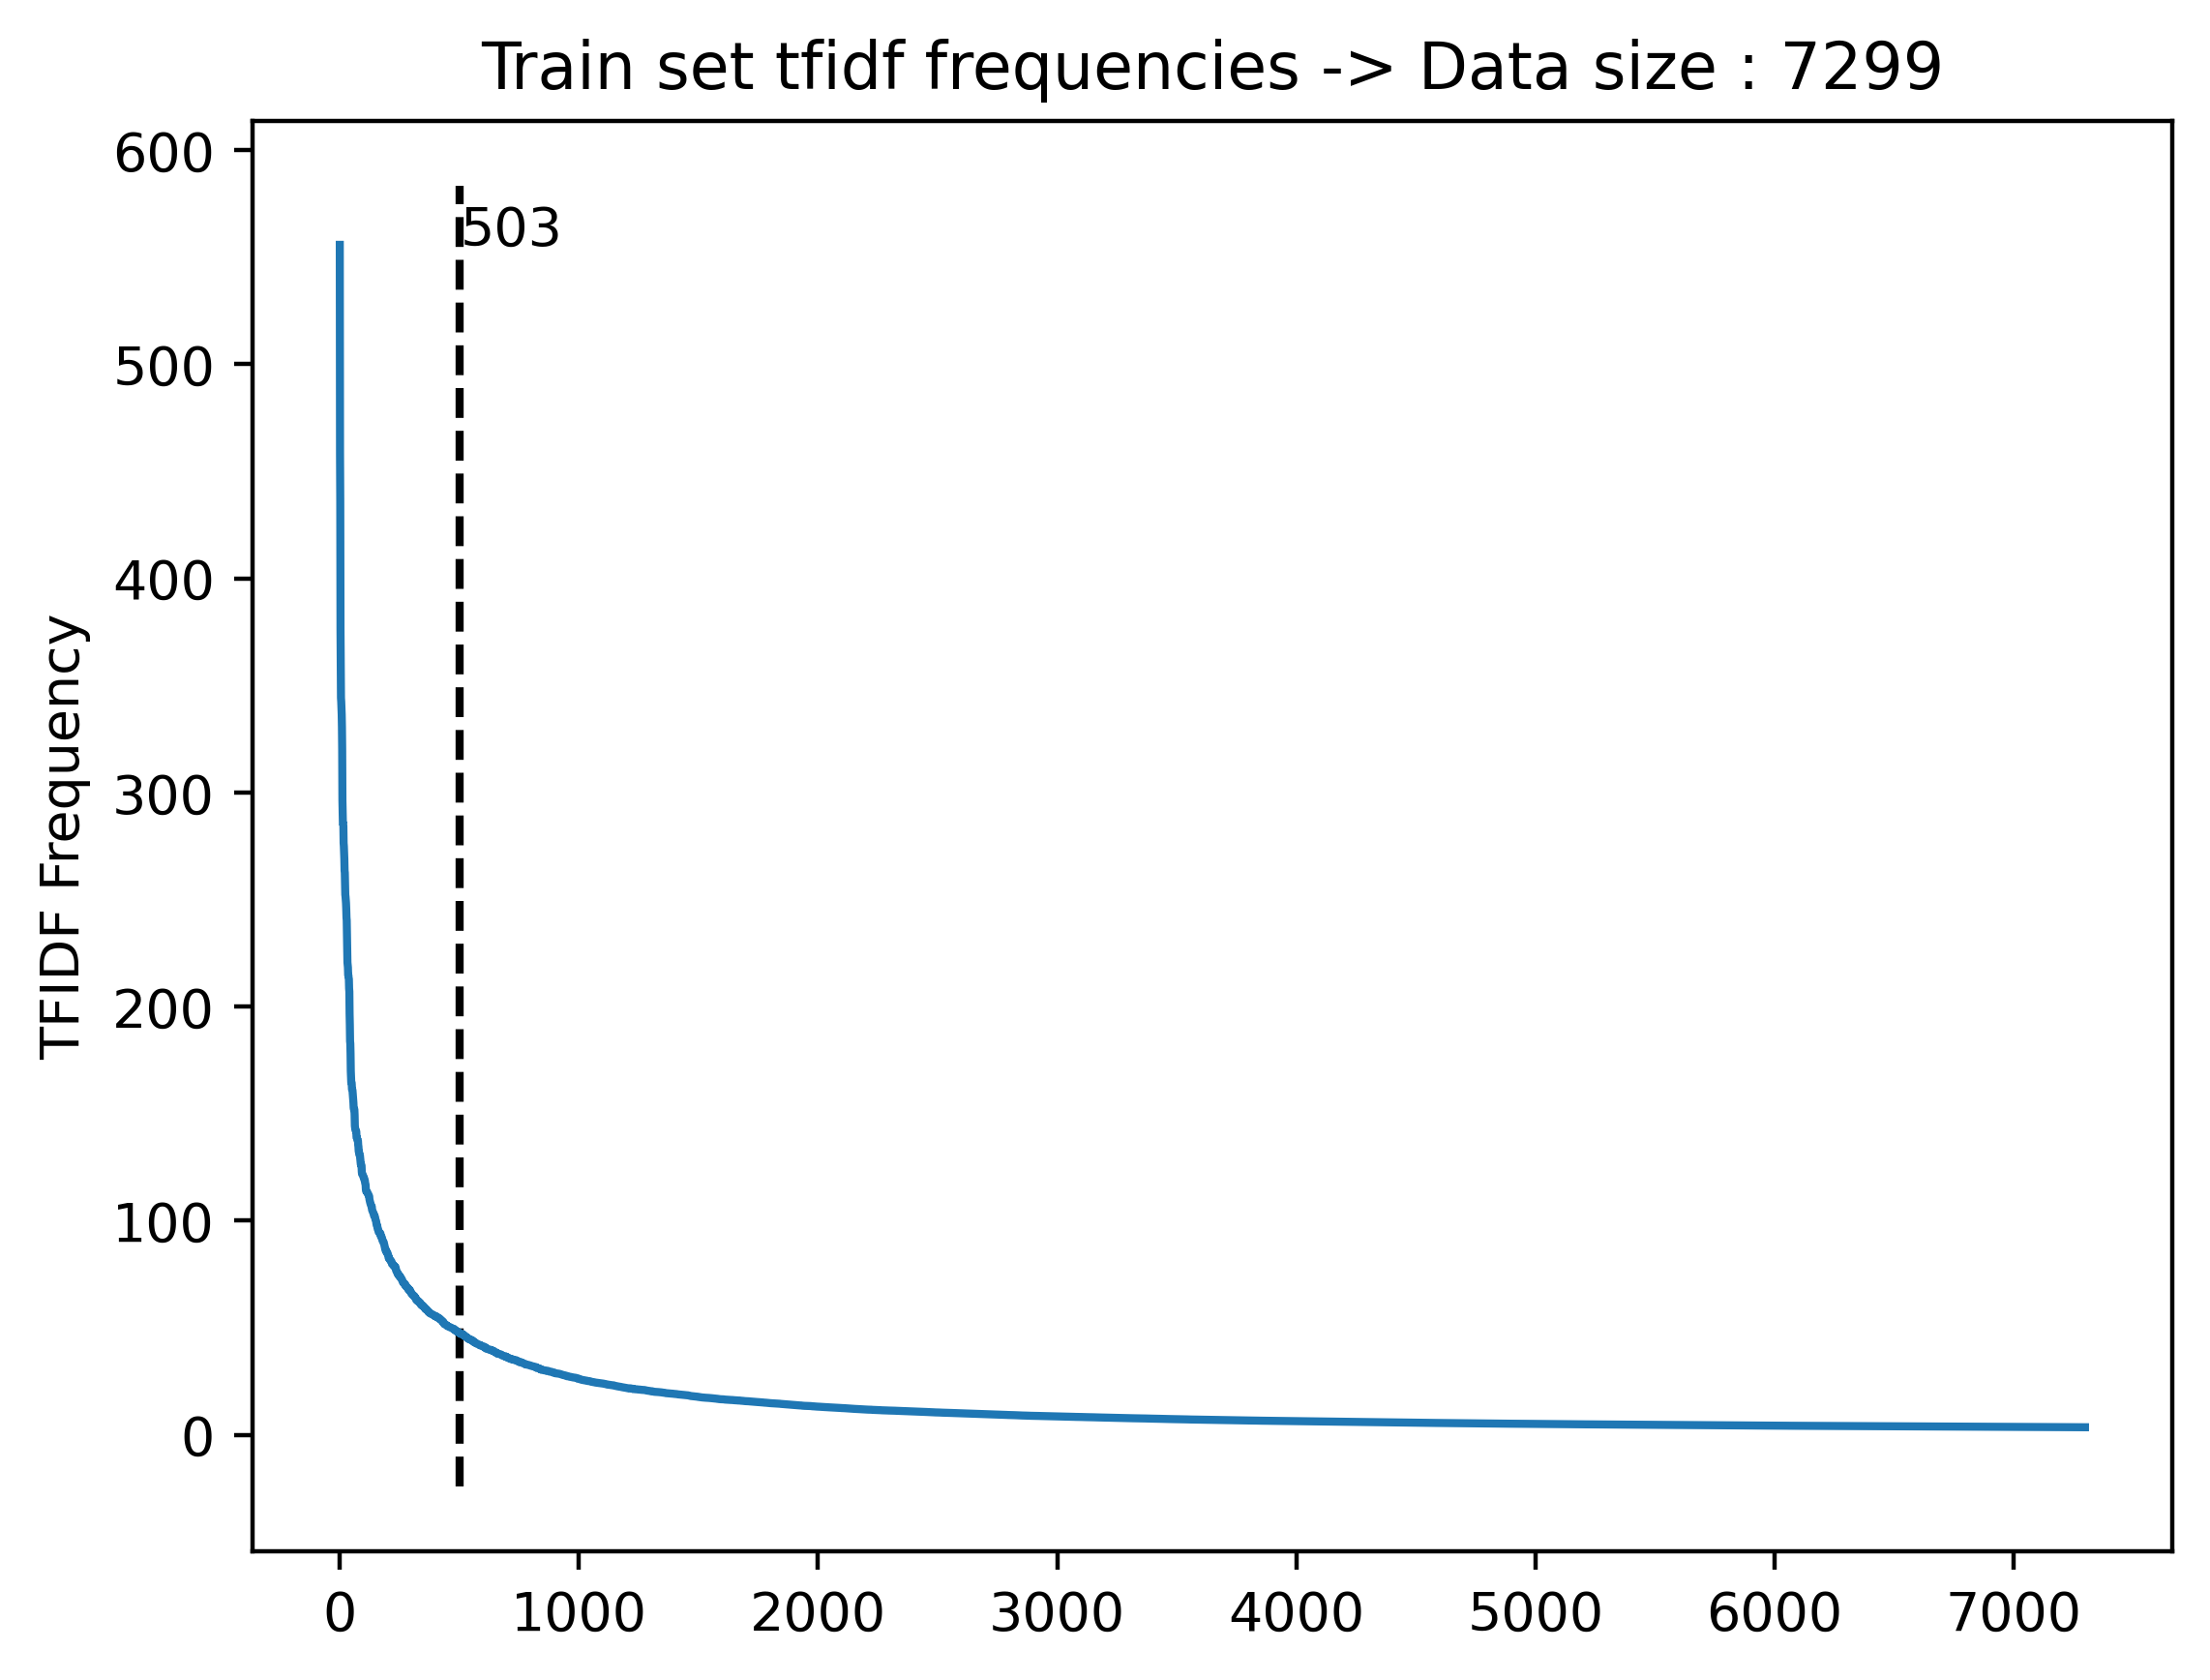
\includegraphics[width=0.5\textwidth,keepaspectratio]{figures/data_size_503.png}
\caption{Frequências TF*IDF do corpus reduzido ordenados de forma decrescente com o \textit{knee\textunderscore{point}}}
\label{diagram:data_second_knee}
\centering
\end{center}
\end{figure}

Como se pode observar, caso a segmentação de dados chegue ao fim, na ultima iteração deste procedimento, o numero de \textit{features} é muito reduzido (11), o que não permite ao modelo obter informação suficiente sobre os documentos. Para evitar isto, foi implementado um parâmetro de limite, que define o numero mínimo de termos que o vocabulário deve ter. Por exemplo, se o limite for de 90 termos, o processo terminaria no terceiro gráfico da figura \ref{diagram:data_all_knee} e o vocabulário ficaria com 93 termos.

\begin{figure}[t]
\begin{center}
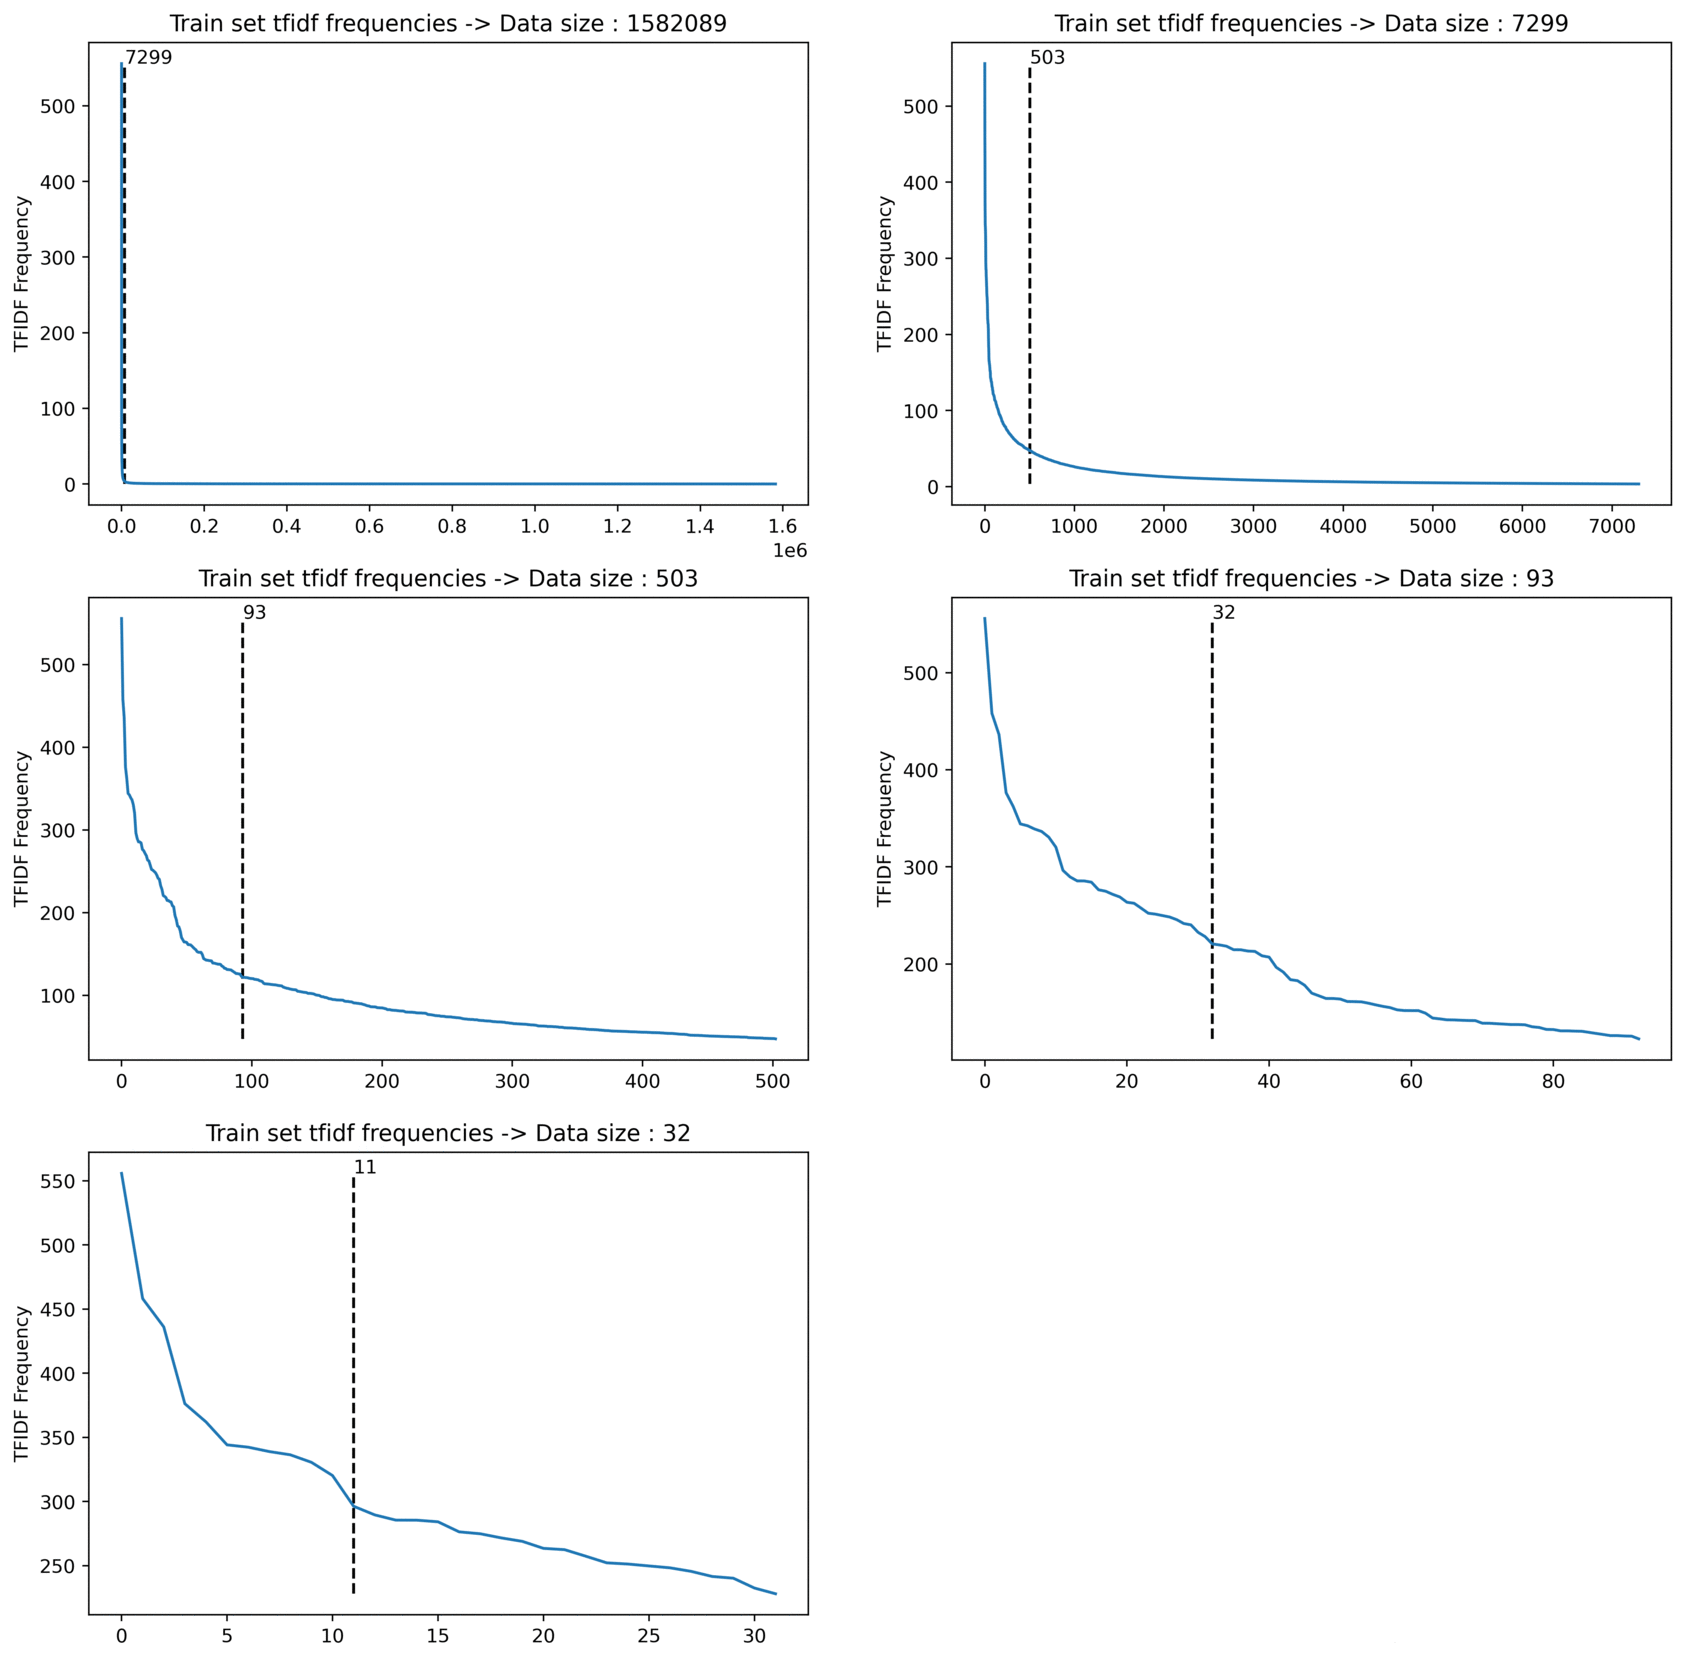
\includegraphics[width=0.5\textwidth,keepaspectratio]{figures/all_graphics.png}
\caption{Sequencias de graficos frequências TF*IDF com o \textit{knee\textunderscore{point}}}
\label{diagram:data_all_knee}
\centering
\end{center}
\end{figure}

\item \textbf{Conversão da lista de \textit{tokens} para uma matriz de \textit{TF features} usando o novo vocabulário reduzido na etapa anterior} 

Após o processo de segmentação do vocabulário, o numero de \textit{features} ideal está definido (500-700 termos).

Neste processo foi usado o algoritmo \textit{TF}, que mapeia a frequência de um termo tendo em conta o vocabulário definido anteriormente. Com estes valores temos uma noção de quantas vezes as palavras mais importantes são usadas nos documentos do \textit{dataset}.
\end{enumerate}

Após estas etapas os dados estão prontos para transitar para a parte de treino.


\subsection{Divisão dos dados para o estudo}
\label{subsub:data_initial_division}

Apesar do \textit{dataset} original possuir 1013 classes distintas, por uma questão de \textit{hardware constraints}, decidimos usar apenas 50 para realizar o nosso estudo, sendo que a selecção das mesmas foi feita de forma aleatória. Desta forma, todo o trabalho foi feito usando 50 mil exemplos de \textit{posts} distintos, já que cada classe, como já referido, possui 1000 amostras. 

Como recomendação dos proprietários do \textit{dataset}, usamos a divisão 80\%-20\% para dados de treino/\textit{cross validation} e de teste, já que os dados originais se encontravam organizados de forma a que, com esta divisão, houvessem exactamente 800 amostras para treino/\textit{cross validation} e 200 amostras para teste em cada classe distinta. Nos gráficos da figura \ref{fig:data_distribution} é possível verificar a uniformidade esta distribuição.


\begin{figure*}[!t]
	\centering
	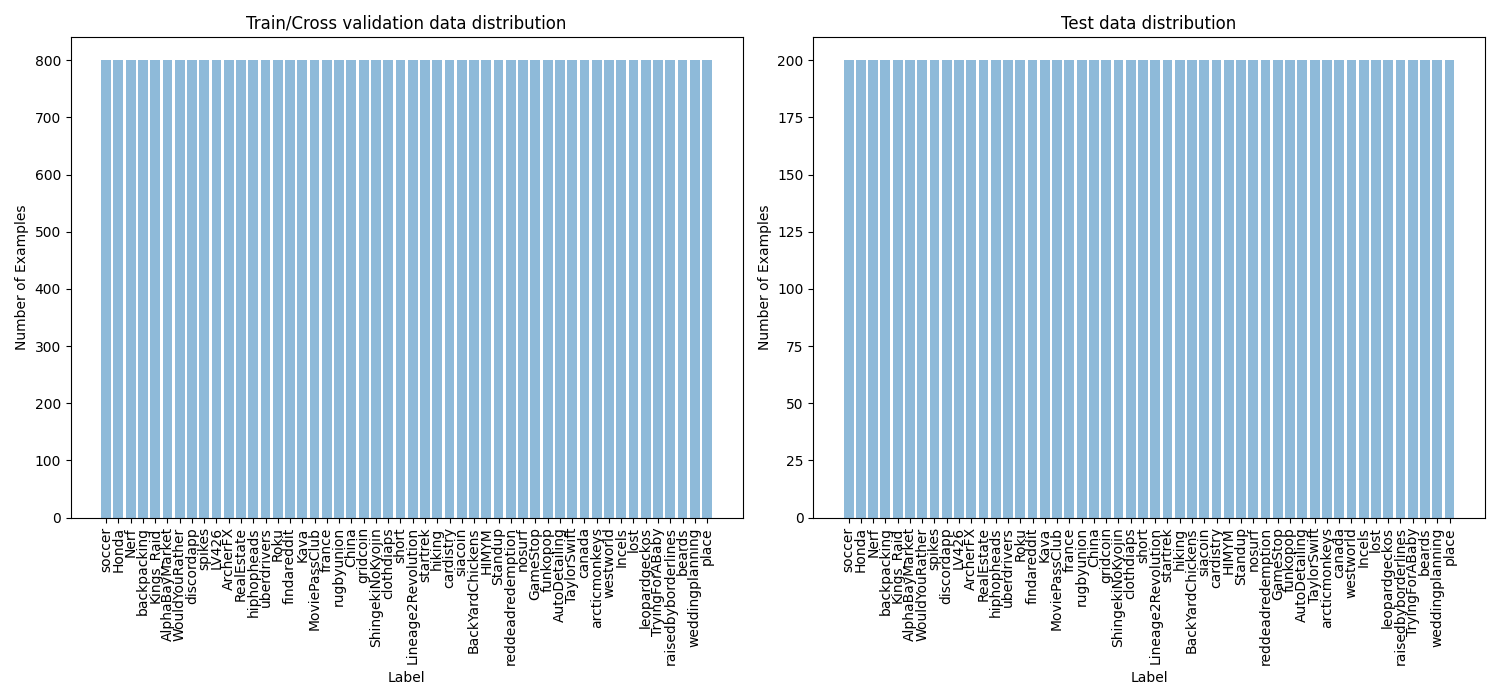
\includegraphics[width=\textwidth]{all_distribution}
	\caption{Distribuição de dados por \textit{label} por \textit{dataset}.}
	\label{fig:data_distribution}
\end{figure*}

\section{Análise de sentimento como processo de complementação}

Com a análise prévia dos textos fornecidos no \textit{dataset} e com o conhecimento prévio da plataforma \textit{Reddit}, foi observado que os textos têm alguma complexidade e variância no que toca à formalidade do mesmo.
Para facilitar a compreensão de um determinado texto, foi usado um modelo pré-treinado capaz de qualificar um texto em positivo, negativo e neutro. O modelo usado foi disponibilizado pelo grupo \textit{VADER Sentiment Analysis} \cite{vader}.

Como esta etapa foi usada como processo de complementação, este modelo foi aplicado a todos os textos do \textit{dataset}, com objectivo de mapear um valor capaz de qualificar o sentimento dos textos. Ou seja, o modelo possui como dados de entrada as matrizes transformadas no processo descrito na secção de pré-processamento e um valor que transmite o sentimento do texto.

Para efeitos de aprovação, o gráfico \ref{diagram:Sentiment_vs_no_sentiments} apresenta os valores da \textit{accuracy} do mesmo modelo com e sem a \textit{feature} que transmite o sentimento do texto. Como se pode observar, o modelo que dispunha da indicação do sentimento de texto obteve uma melhor performance em termos de \textit{accuracy} em ambos os conjuntos, o que indica que este valor é uma boa adição para a performance do modelo, já que ajuda a descodificar a parte semântica do texto que não é observável apenas com a noção de \textit{tokens}.


\begin{figure}[!t]
\begin{center}
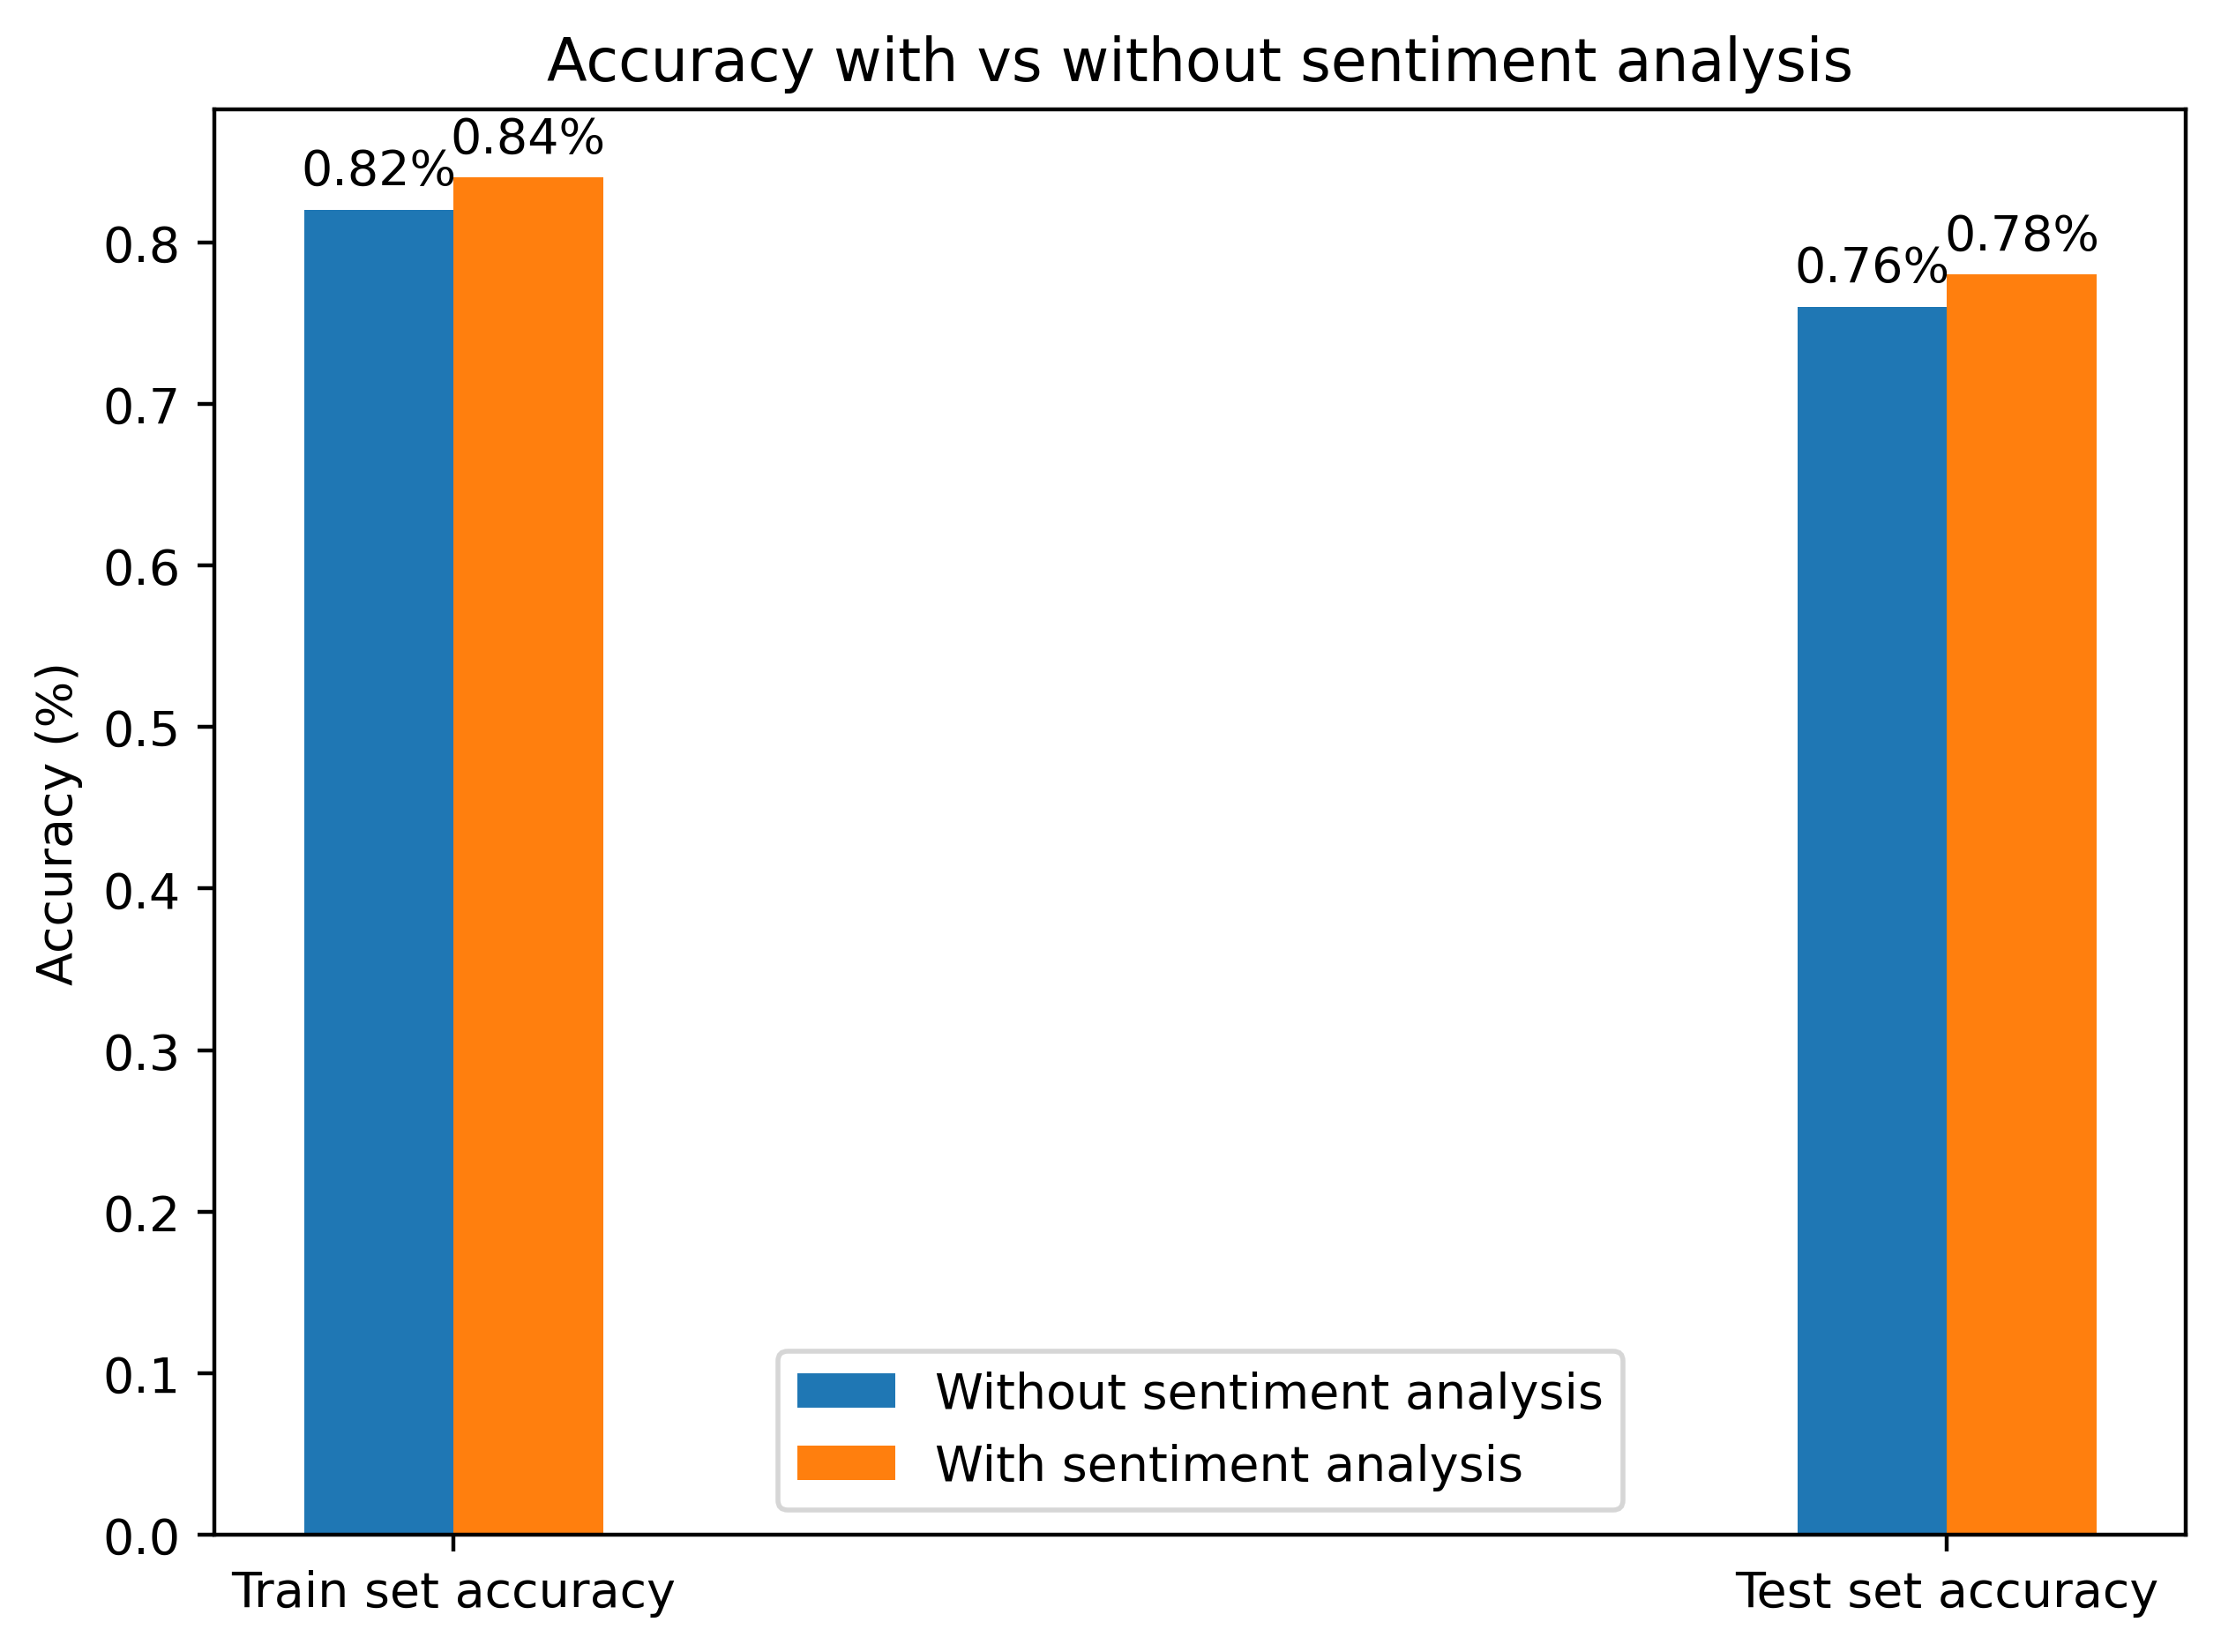
\includegraphics[width=0.5\textwidth,keepaspectratio]{figures/sentiment_vs_no_sentiment.png}
\caption{\textit{Accuracy} do mesmo modelo \textbf{com e sem} o valor que transmite o sentimento do texto}
\label{diagram:Sentiment_vs_no_sentiments}
\centering
\end{center}
\end{figure}

\section{Estudo com Redes Neuronais}
Sendo que o pressuposto das Redes Neuronais é que tenham um bom desempenho, em termos da qualidade da prestação de modelos treinados usando o mesmo, foi a primeira abordagem que decidimos dar ao problema.

\subsection{Estrutura usada}
Apesar do \textit{dataset} ter dimensões consideráveis para o \textit{hardware} disponível, consideramos que este problema consegue ser resolvido com uma rede neuronal "normal". O uso de uma rede convolucional neste problema acaba por ser evitado, pois na fase de pré-processamento existem métodos de selecção de \textit{features} suficientes para o modelo ter uma performance boa, não sendo necessário que o modelo tenha a responsabilidade de fazer a procura de \textit{features}.
Então após a experimentação de alguns valores relativos ao número de neurónios e número de \textit{hidden layers} consideramos uma rede neuronal com as seguintes características:

Input \textrightarrow{} 200 Neurónios \textrightarrow{} 100 Neurónios \textrightarrow{} Output

Para além disso, a inicialização dos \textit{weights} foi feita usando o  \texit{glorot uniform initializer} \cite{Glorot_Uniform}. Os valores dos hiperparâmetros usado foram:
\begin{itemize}
    \item Número de \textit{features} (termos do vocabulário): 500-600
    \item Número de \textit{epochs} = 200
    \item \textit{Batch size} = 500
    \item \textit{Activation function} 
        \begin{itemize}
            \item \textit{Hidden Layers}: \textit{Relu} \cite{relu_function}
            \item \textit{Output Layer}: \textit{Softmax} \cite{softmax_function}
        \end{itemize}
    \item \textit{Optimizer}: \textit{Adam} \cite{adam_optimizer}
    \item \textit{Loss function}: \textit{Categorical crossentropy} \cite{categorical_crossentropy_optimizer}
\end{itemize}


Desde o inicio da implementação deste modelo foi usado o processo de treino-validação utilizando o \textbf{\textit{K-Fold Cross validation}}. Este método tem um parâmetro k que define o número de divisões que o conjunto será sujeito, cada porção segmentada é intitulada de \textit{fold}. No processo de treino todos os \textit{folds} são usados para teste uma vez, sendo que os outros restantes k-1 \textit{folds} são usados para o processo de treino. Neste estudo, o valor de \textit{k} definindo foi 5 (\textbf{\textit{K\textunderscore{fold}} com 5 \textit{splits}}).
Ainda foi adicionado um \textit{callback} de \textit{Early stopping} com objectivo de suspender o treino quando o parâmetro a ser monitorizado (neste caso o \textit{validation accuracy}) para de melhorar.


\subsection{Resultados obtidos}

Após as condições definidas anteriormente decidimos então testar a performance do modelo. 
Obtivemos então os seguintes valores de \textit{accuracy}, após retreino do modelo:

\begin{itemize}
        \item \textit{Train Score}: 0.82
        \item \textit{Test Score}: 0.71
\end{itemize}


Como se pode observar pelos resultados e pelos gráficos \ref{diagram:accuracy_fold_first} e \ref{diagram:accuracy_retrain}, o modelo tem tendência a realizar o fenómeno de \textit{overfit} e portanto as próximas subsecções têm como objectivo explicar os mecanismos usados para evitar este fenómeno. Apenas de salientar que devido ao \textit{callback} de  \textit{early stopping}, o treino é parado pois a \textit{accuracy} do conjunto de validação não aumenta, o que acaba por evitar uma maximização do fenómeno de \textit{overfit}.



\begin{figure}[t]
\begin{center}
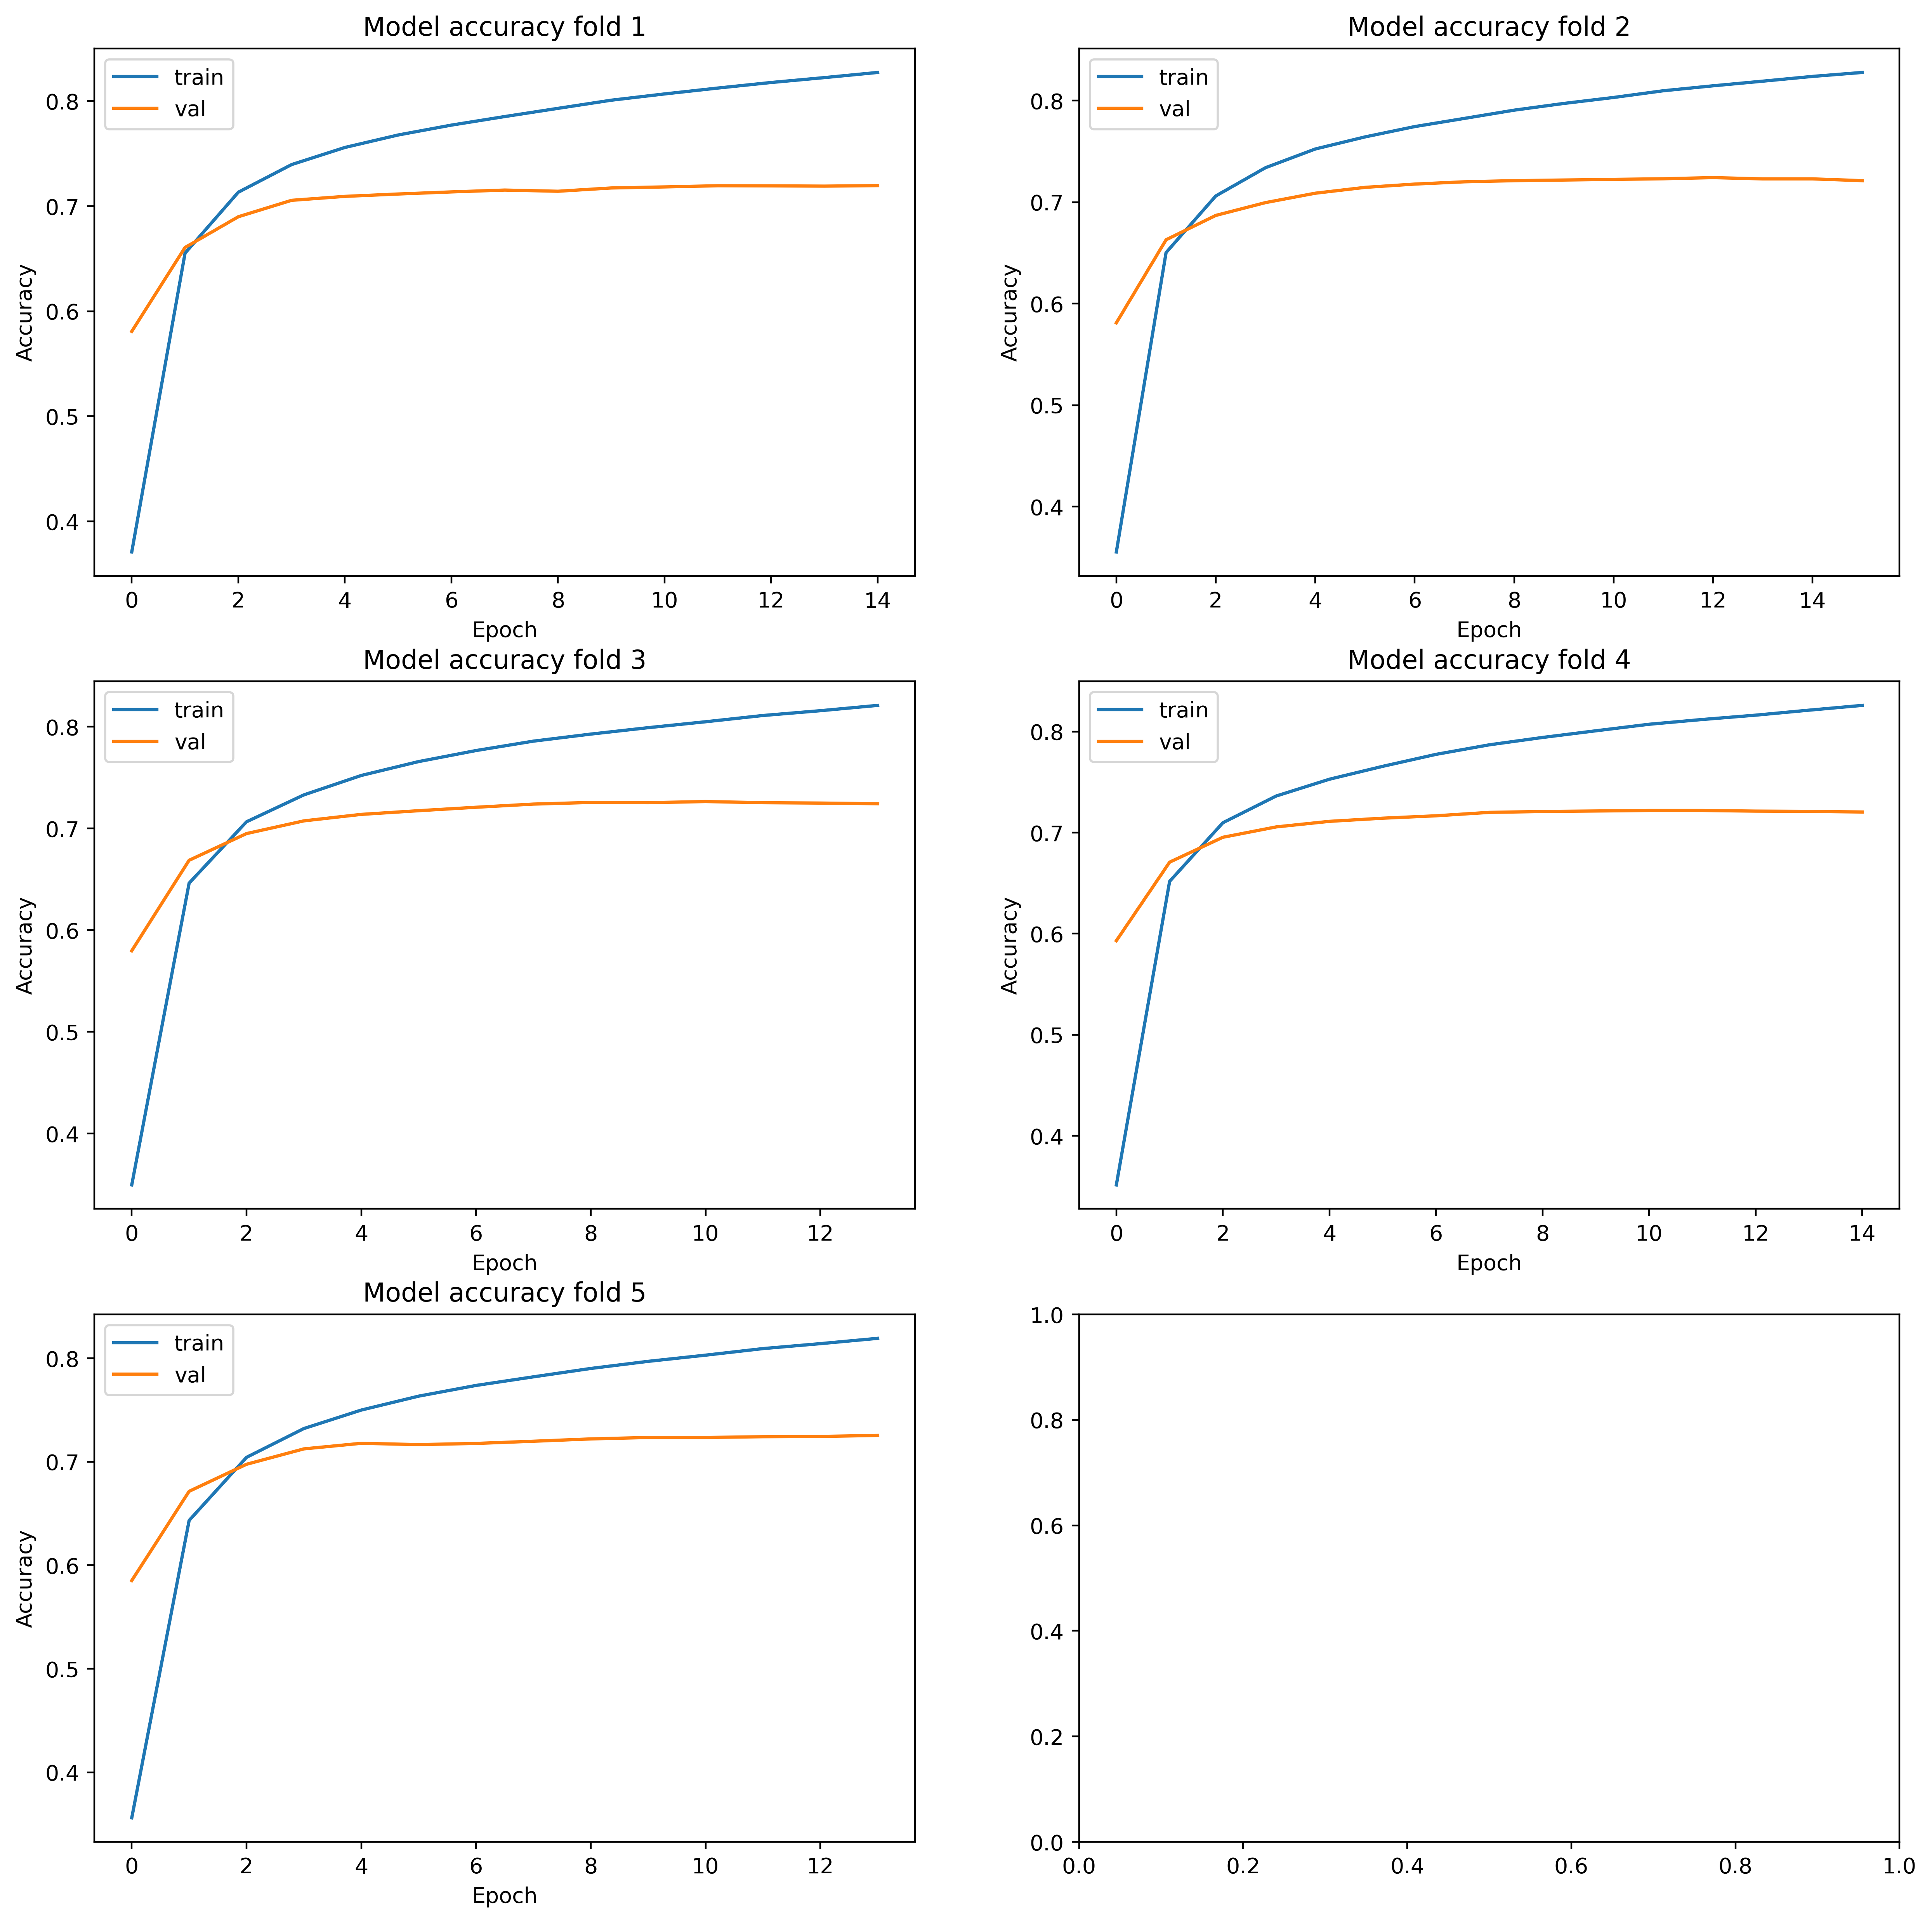
\includegraphics[width=0.5\textwidth,keepaspectratio]{figures/merged_fold_graphics_first.png}
\caption{\textit{Accuracy function} de cada \textit{fold}}
\label{diagram:accuracy_fold_first}
\centering
\end{center}
\end{figure}

\begin{figure}[t]
\begin{center}
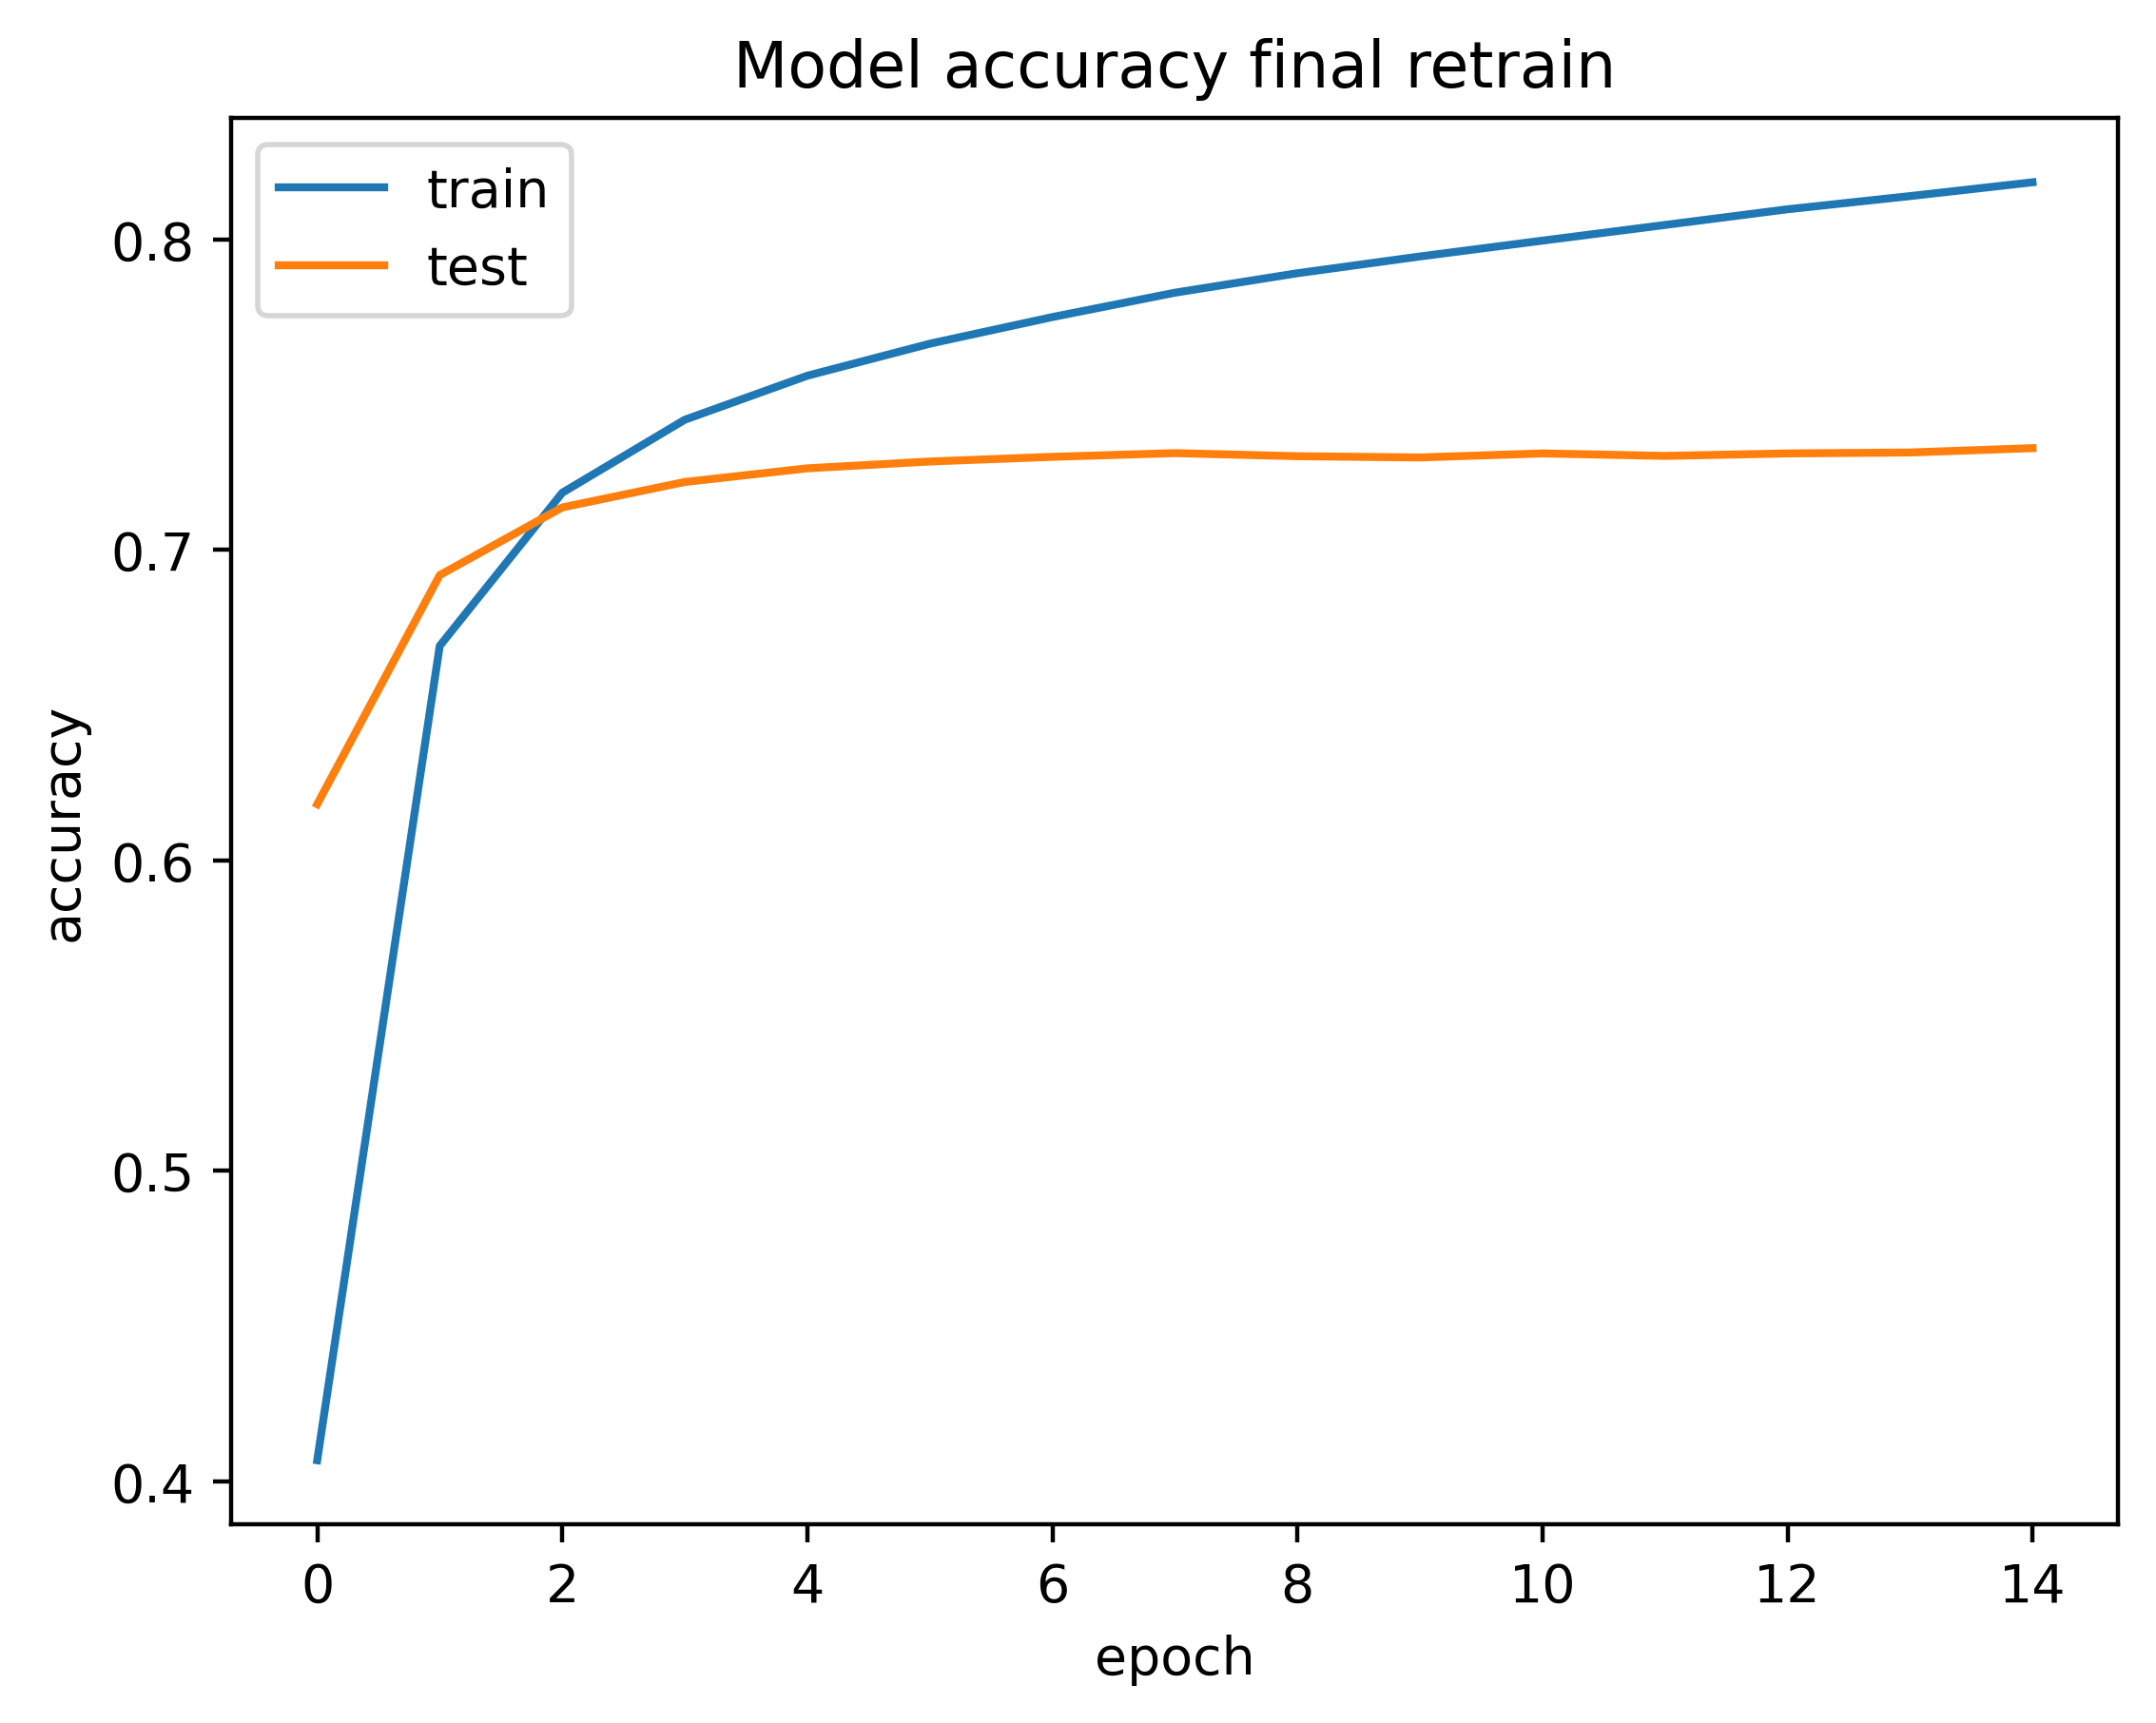
\includegraphics[width=0.5\textwidth,keepaspectratio]{figures/50_final_png_first.png}
\caption{\textit{Accuracy function} após re-treino com o conjunto de treino na totalidade}
\label{diagram:accuracy_retrain}
\centering
\end{center}
\end{figure}

\subsection{Melhoria do modelo}

Para evitar o fenómeno de \textit{overfit} decidimos acrescentar uma função de \textit{regularização} nos pesos, \textit{L2 regularization penalty} \cite{l2_regularizer}, nas \textit{hidden layers}. Basicamente a regularização evita o fenómeno de \textit{overfit}, restringindo os valores dos pesos, evitando que o modelo se adapte demasiado à forma dos dados de treino.
Para isso o algoritmo de regularização tem um parâmetro que define o impacto da regularização nos termos. Caso o valor seja muito alto, o modelo não tem flexibilidade suficiente para se formatar à forma dos dados, pelo que irá ocorrer o fenómeno de \textit{underfit}. Caso seja muito baixo, o fenómeno de \textit{overfit} pode ocorrer pois o impacto do termo regularizador é fraco.
Como se pode observar no gráfico \ref{diagram:reg_factor}, para valores muito altos do factor de regularização, o modelo não consegue generalizar os dados. O que acabou por se tornar o melhor parâmetro foi o valor de $0.001$, cuja diferença entre a \textit{accuracy} do conjunto de validação e o conjunto de treino é menor.

Os valores após retreino usando o factor de regularização óptimo definido acima são:
\begin{itemize}
        \item \textit{Train Score}: 0.82
        \item \textit{Test Score}: 0.76
\end{itemize}

Como se pode observar nos gráficos \ref{diagram:accuracy_fold_last}  e \ref{diagram:accuracy_retrain_last}, houve uma melhoria relativamente à \textit{accuracy} em dados nunca vistos pelo modelo, o que indica que o fenómeno de \textit{overfit} diminui, o que consequentemente indica que o modelo obteve uma performance melhor.



\begin{figure}[t]
\begin{center}
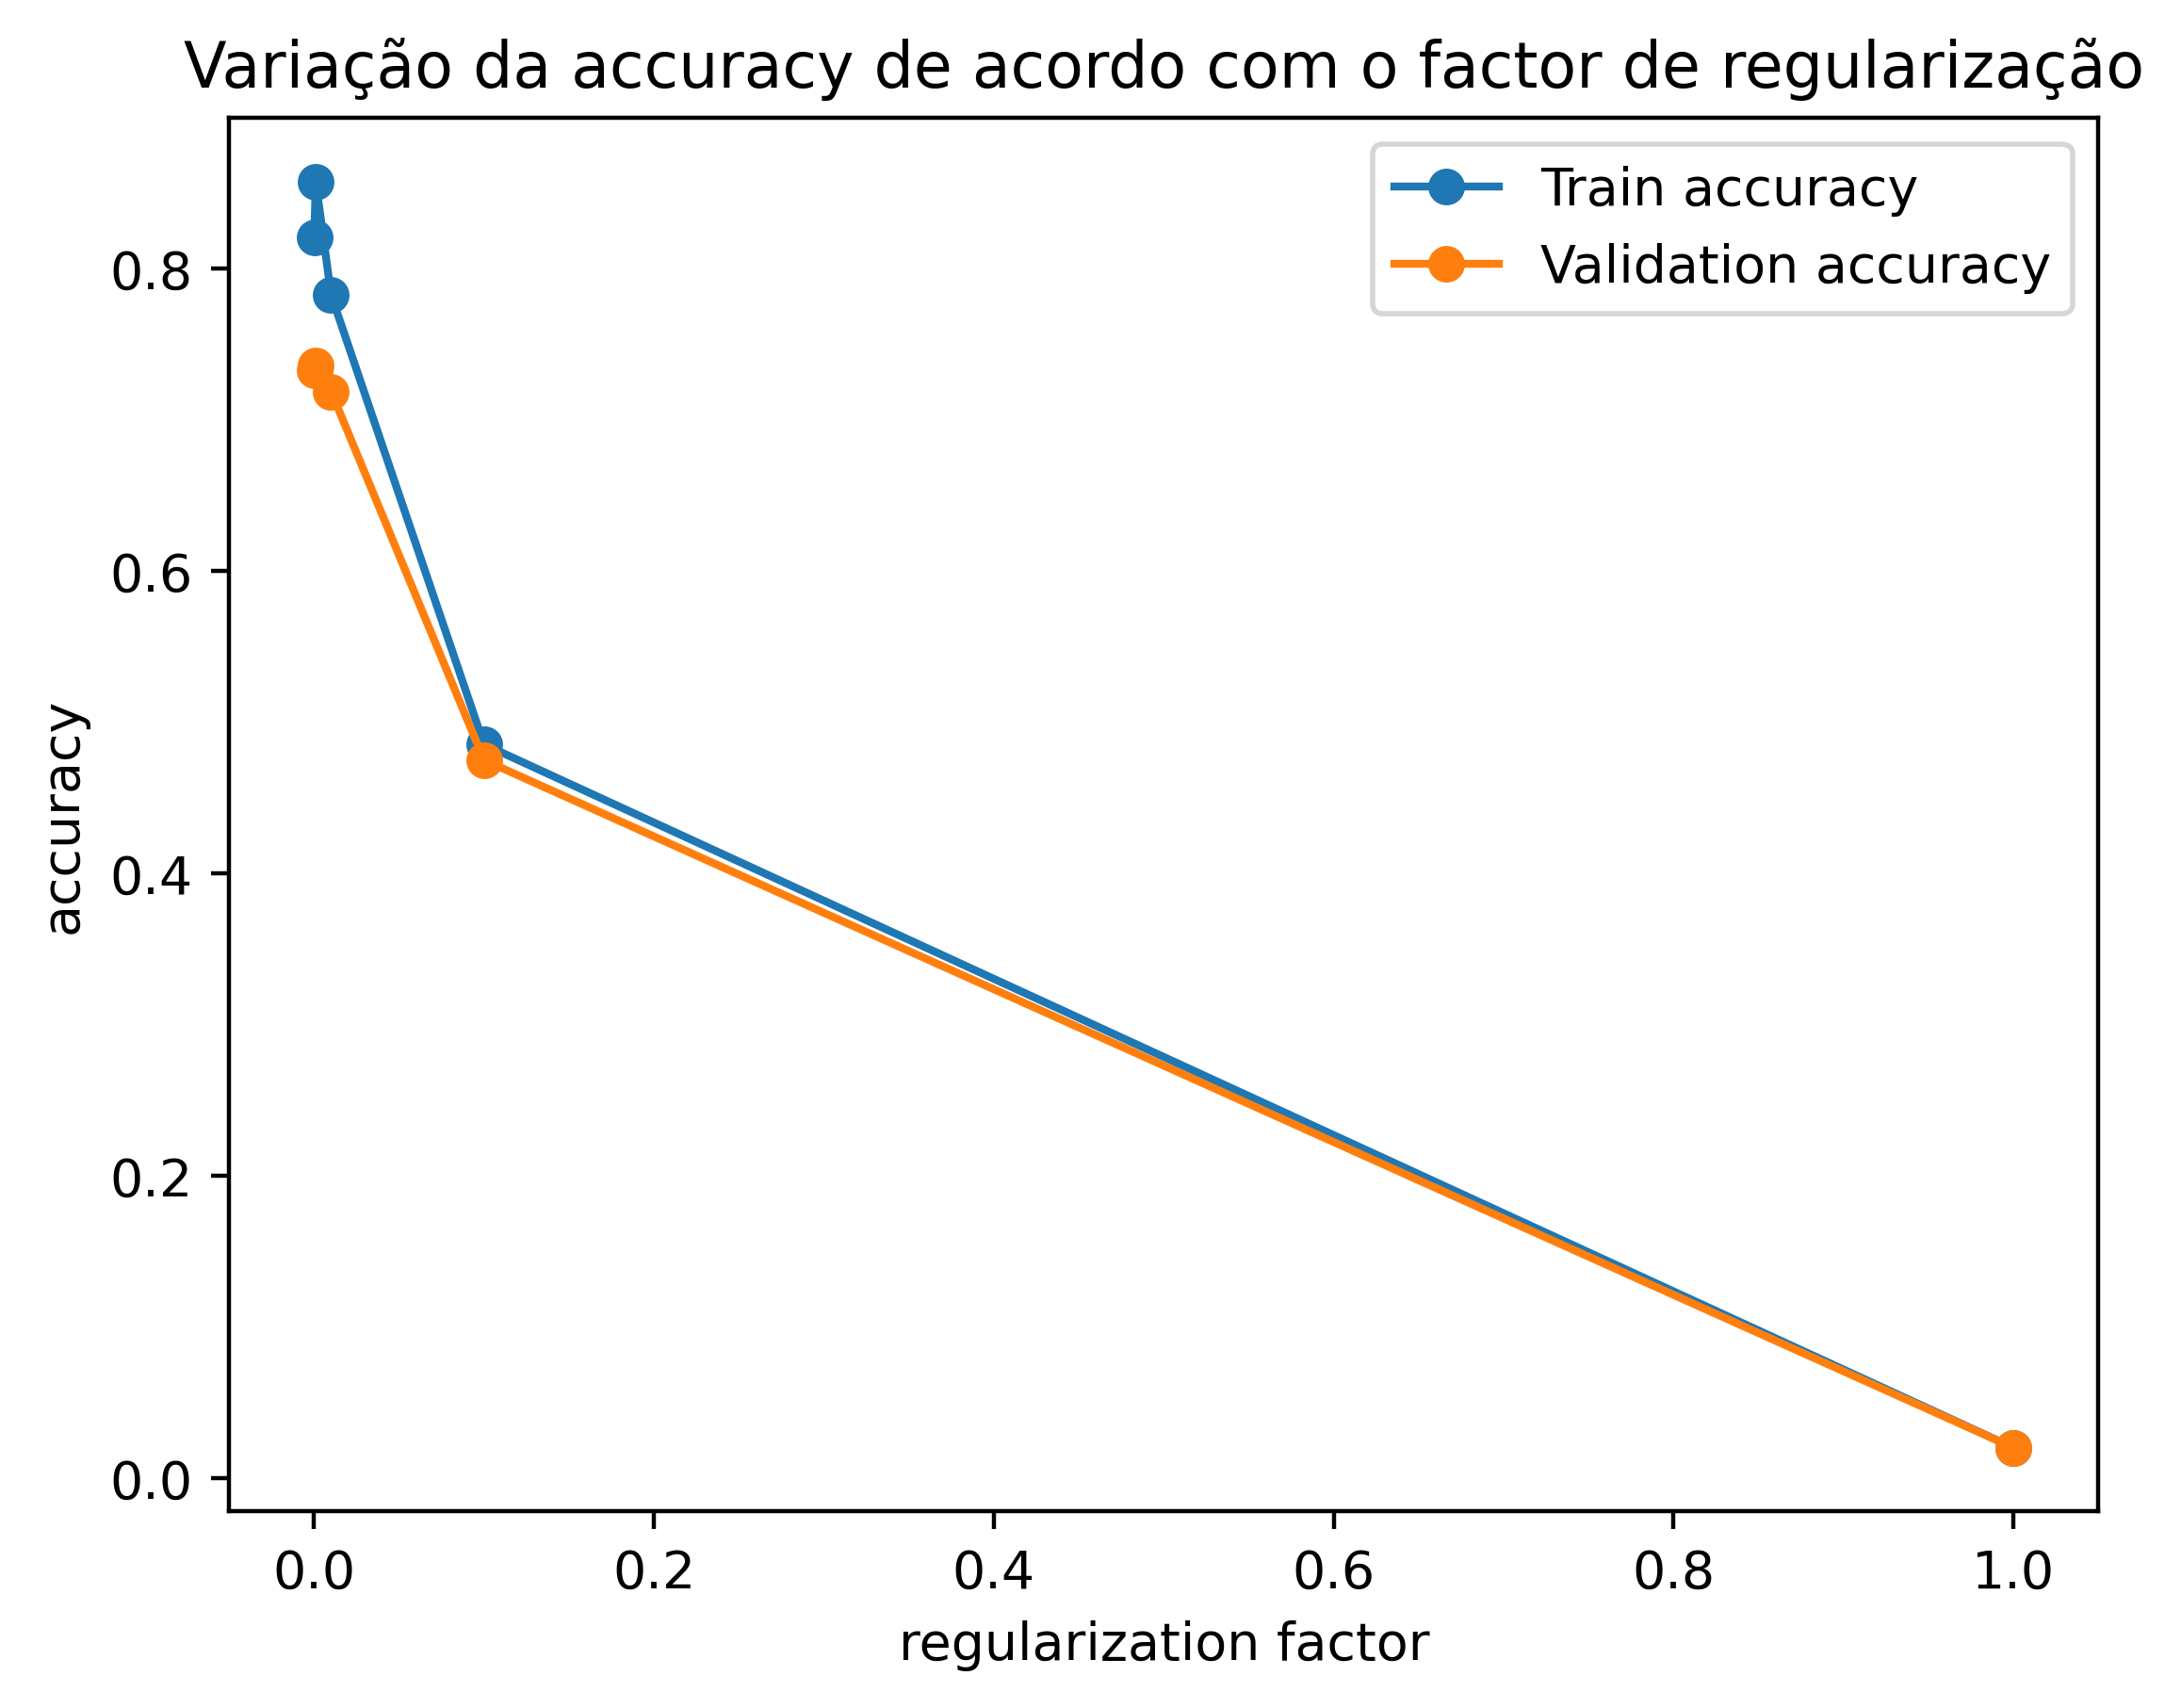
\includegraphics[width=0.5\textwidth,keepaspectratio]{figures/r_Factor.png}
\caption{Variação dos valores de \textit{accuracy} de acordo com o factor de regularização}
\label{diagram:reg_factor}
\centering
\end{center}
\end{figure}


\begin{figure}[t]
\begin{center}
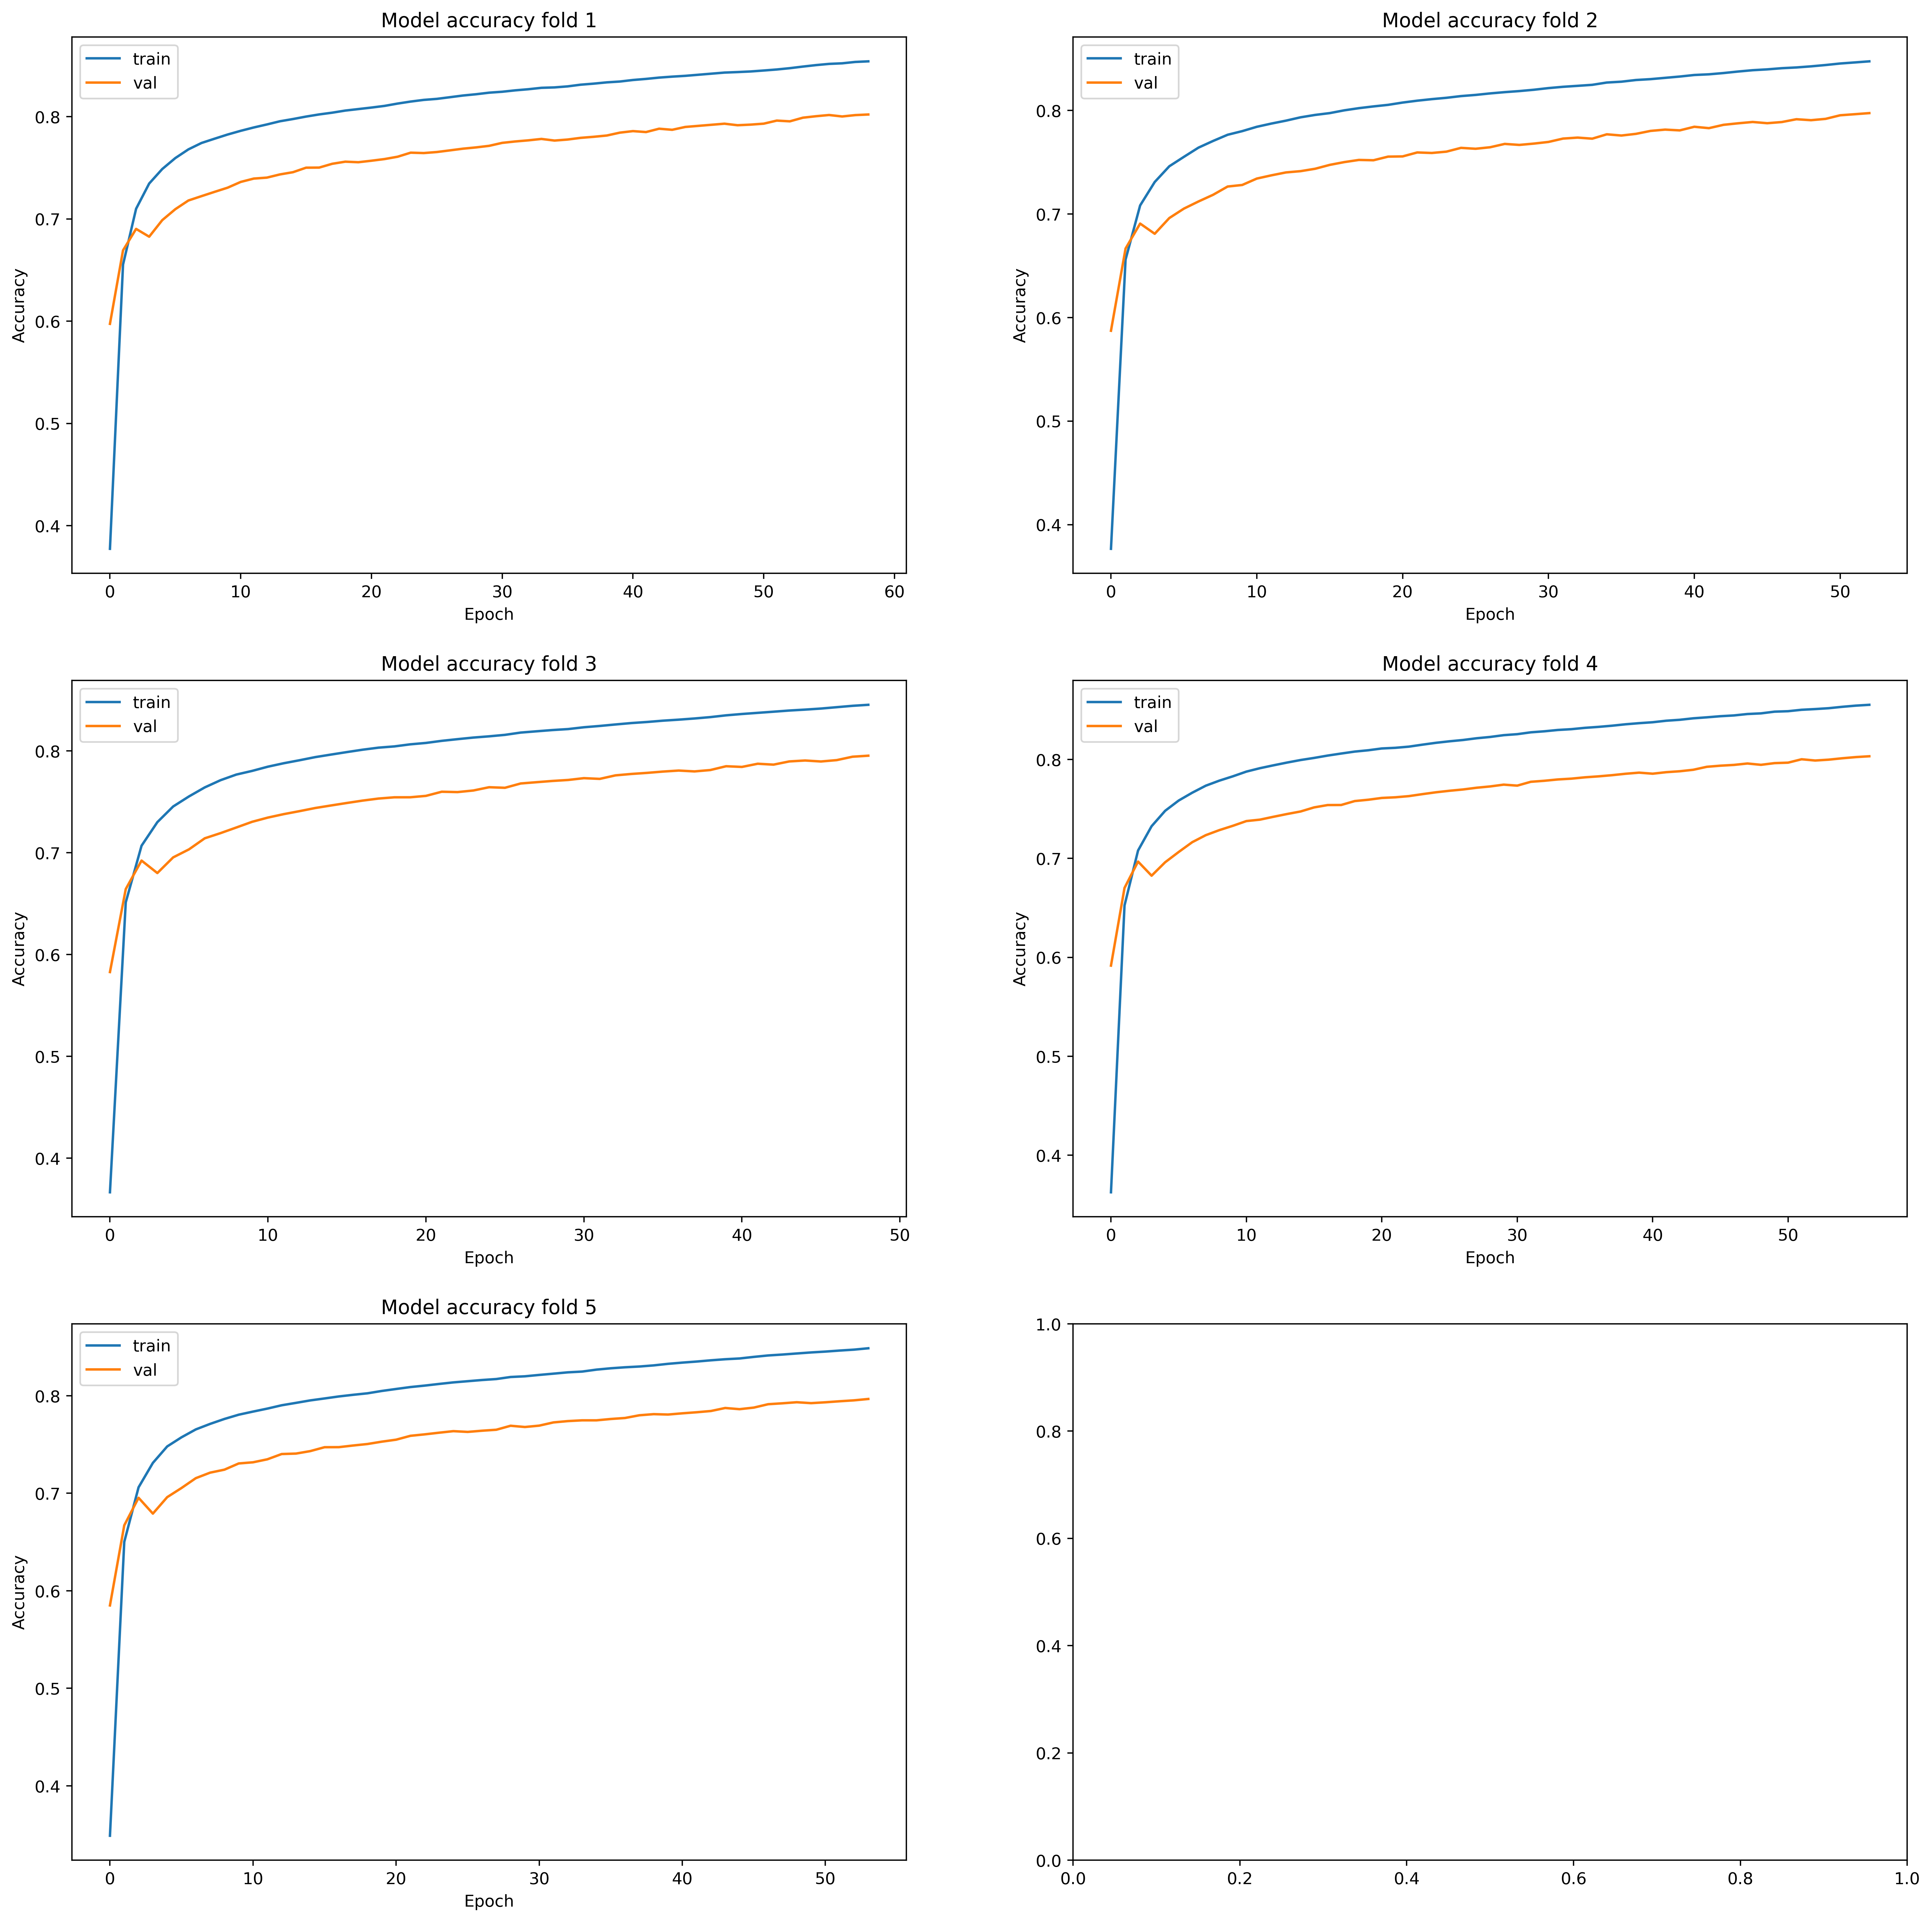
\includegraphics[width=0.5\textwidth,keepaspectratio]{figures/merged_fold_graphics_last.png}
\caption{\textit{Accuracy function} de cada \textit{fold}}
\label{diagram:accuracy_fold_last}
\centering
\end{center}
\end{figure}




\begin{figure}[t]
\begin{center}
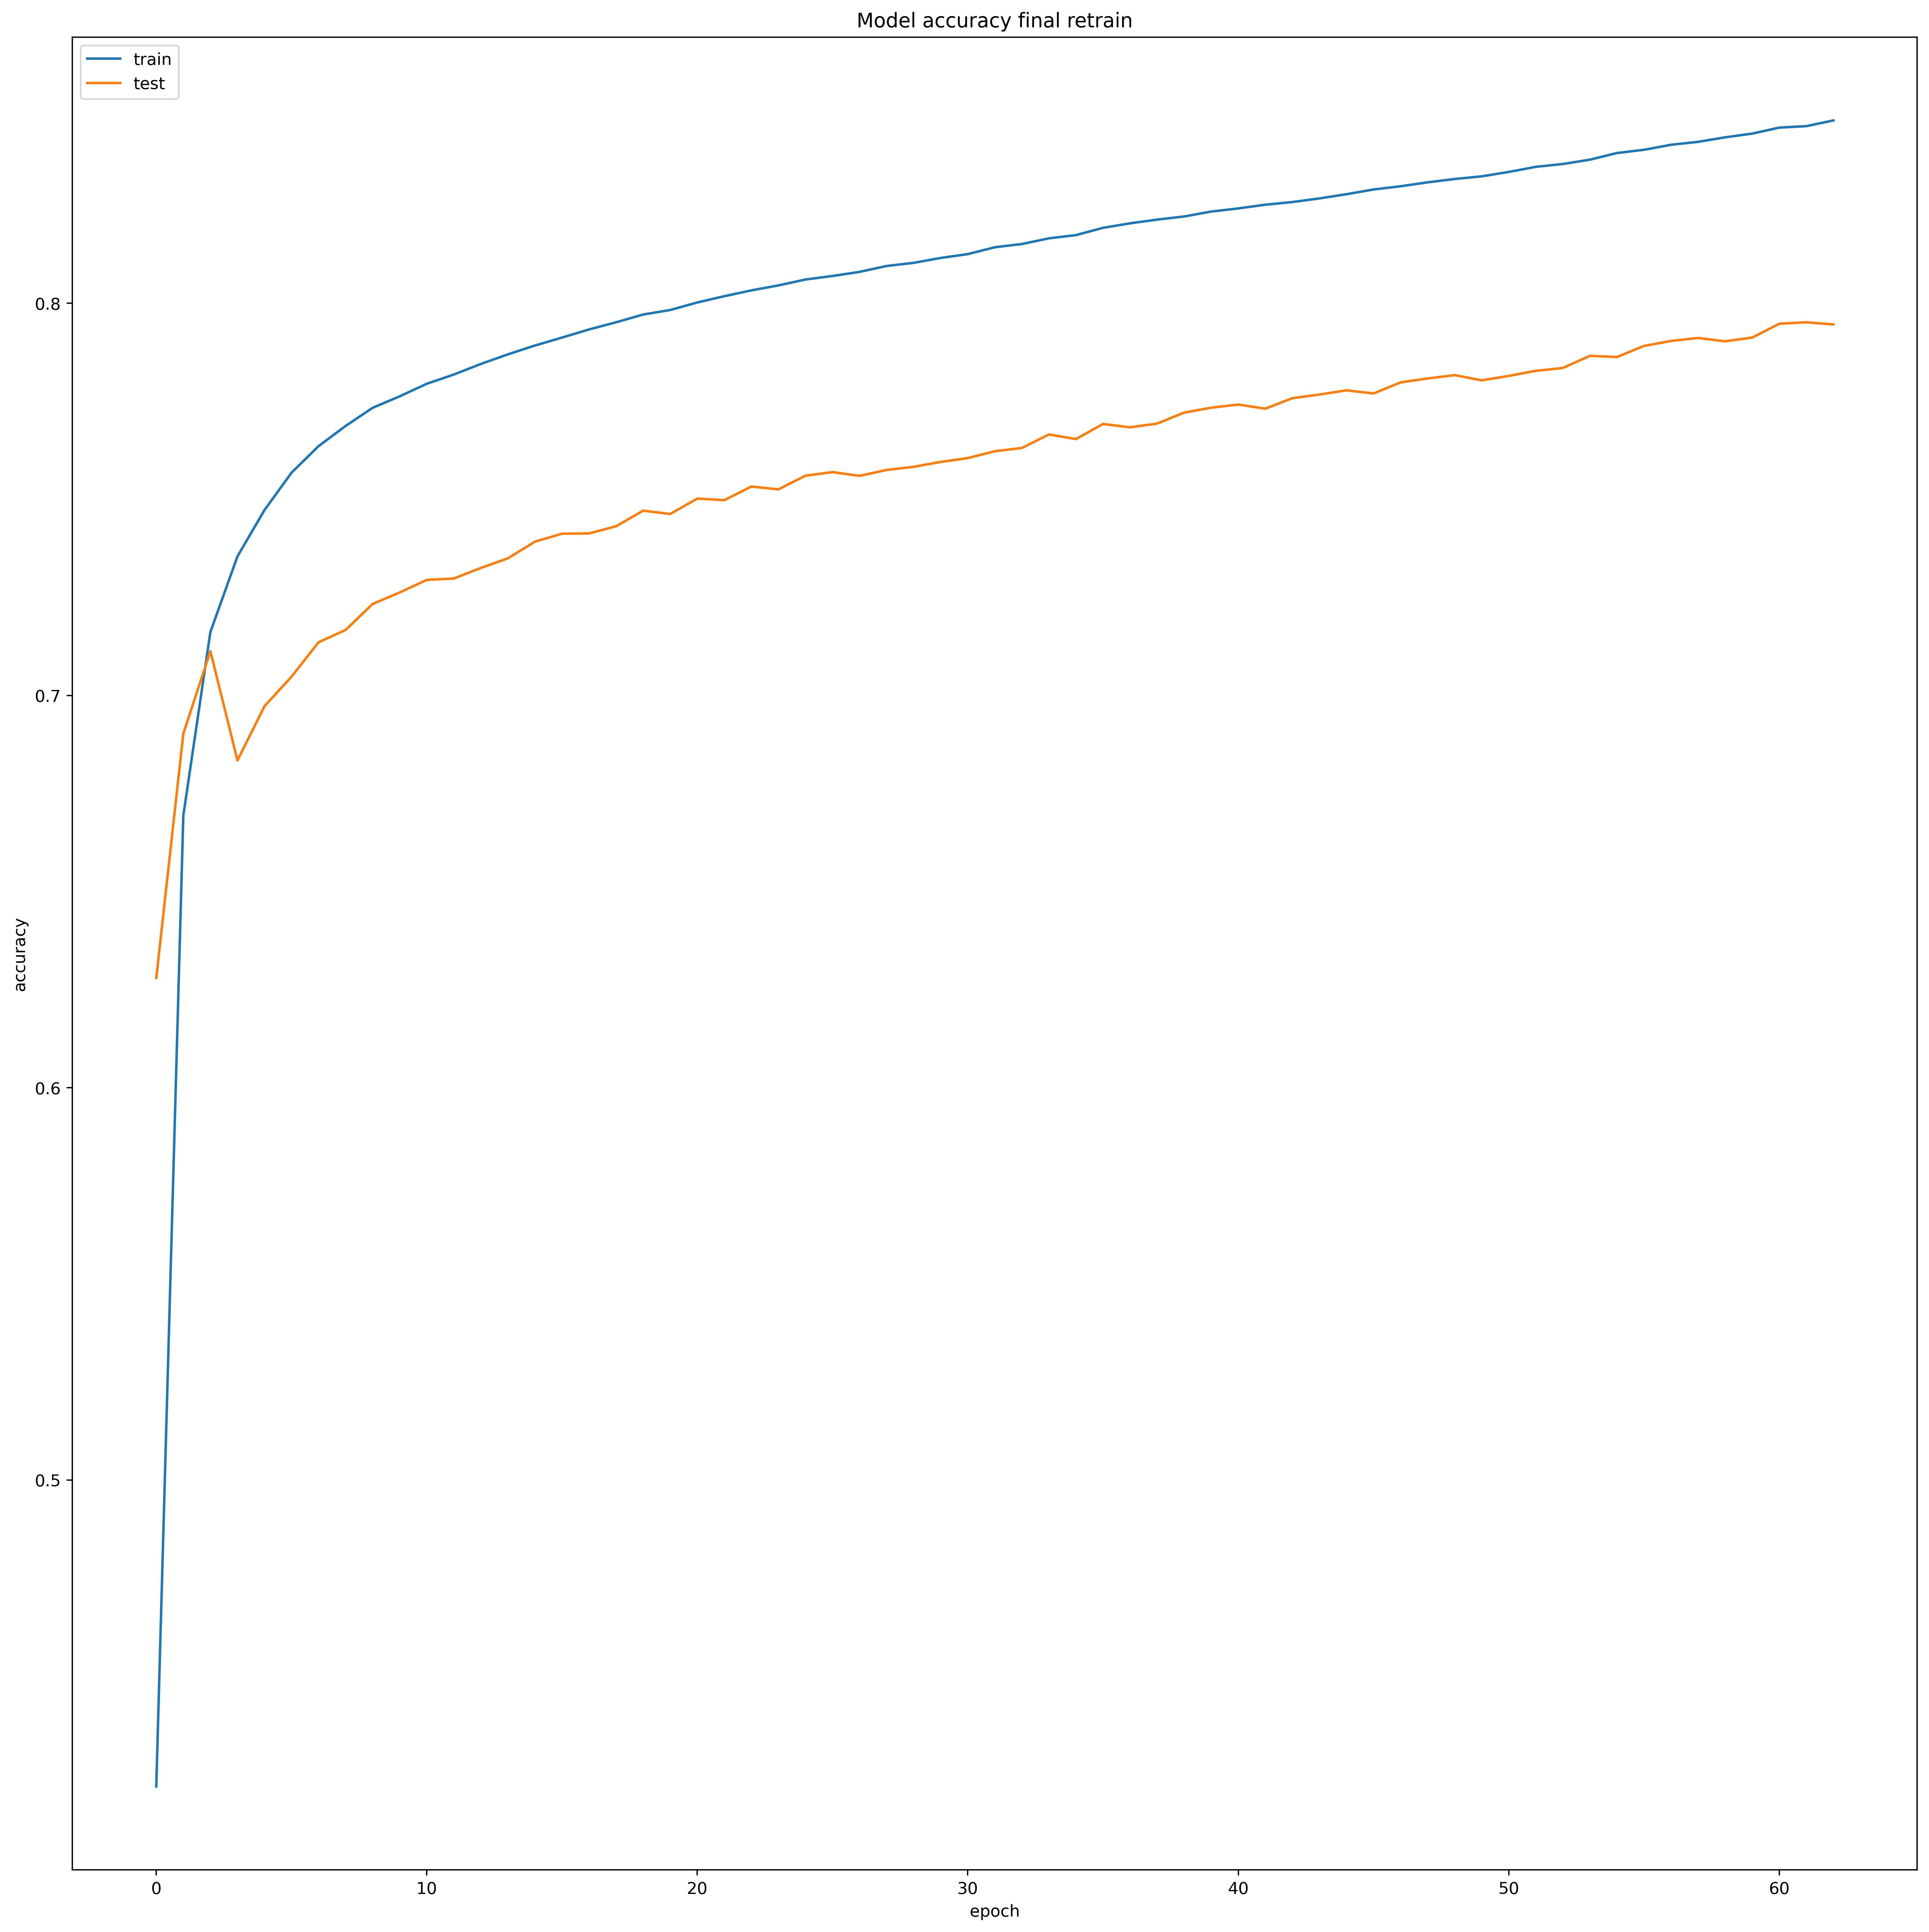
\includegraphics[width=0.5\textwidth,keepaspectratio]{figures/last_retrain.png}
\caption{\textit{Accuracy function} após re-treino com o conjunto de treino na totalidade}
\label{diagram:accuracy_retrain_last}
\centering
\end{center}
\end{figure}

\subsection{Conclusões}
Foram feitos esforços para tentar melhorar a performance deste modelo mas sem sucesso, muito devido à grande dificuldade de \textit{"fine-tune"} das redes neuronais que muito facilmente convergem para o fenómeno de \textit{overfit}.

\section{Estudo com Redes de Bayes}
\label{sec:bayes}

Ao pesquisarmos sobre outros estudos feitos de \textit{machine learning} sob o mesmo \textit{dataset} usado, encontramos a implementação \cite{kaggle_bayes}. Este utilizador do \textit{Kaggle} conseguiu, para 5 classes, obter uma precisão de aproximadamente $0.72$ e uma \textit{accuracy} de aproximadamente $0.61$ \footnote{Apesar do autor não ter documentado esta métrica, nós executamos o código disponibilizado pelo mesmo, obtendo este valor, para 10 mil \textit{features} (não podemos usar mais por falta de recursos físicos)} para os dados de teste.


\subsection{Repartição dos dados}
\label{subsub:bayes_data}

Para além da divisão descrita na secção \ref{subsub:data_initial_division}, fizemos uma segunda divisão nos dados reservados para treino/\textit{cross validation}. Esta divisão foi de realizada de maneira a que obtivéssemos uma distribuição de 60\%-20\%-20\% entre dados de treino, \textit{cross validation} e teste, respectivamente. A distribuição final dos dados por \textit{dataset} pode ser consultada nos gráficos da figura \ref{fig:data_distribution_with_cv}.

\begin{figure*}[!t]
	\centering
	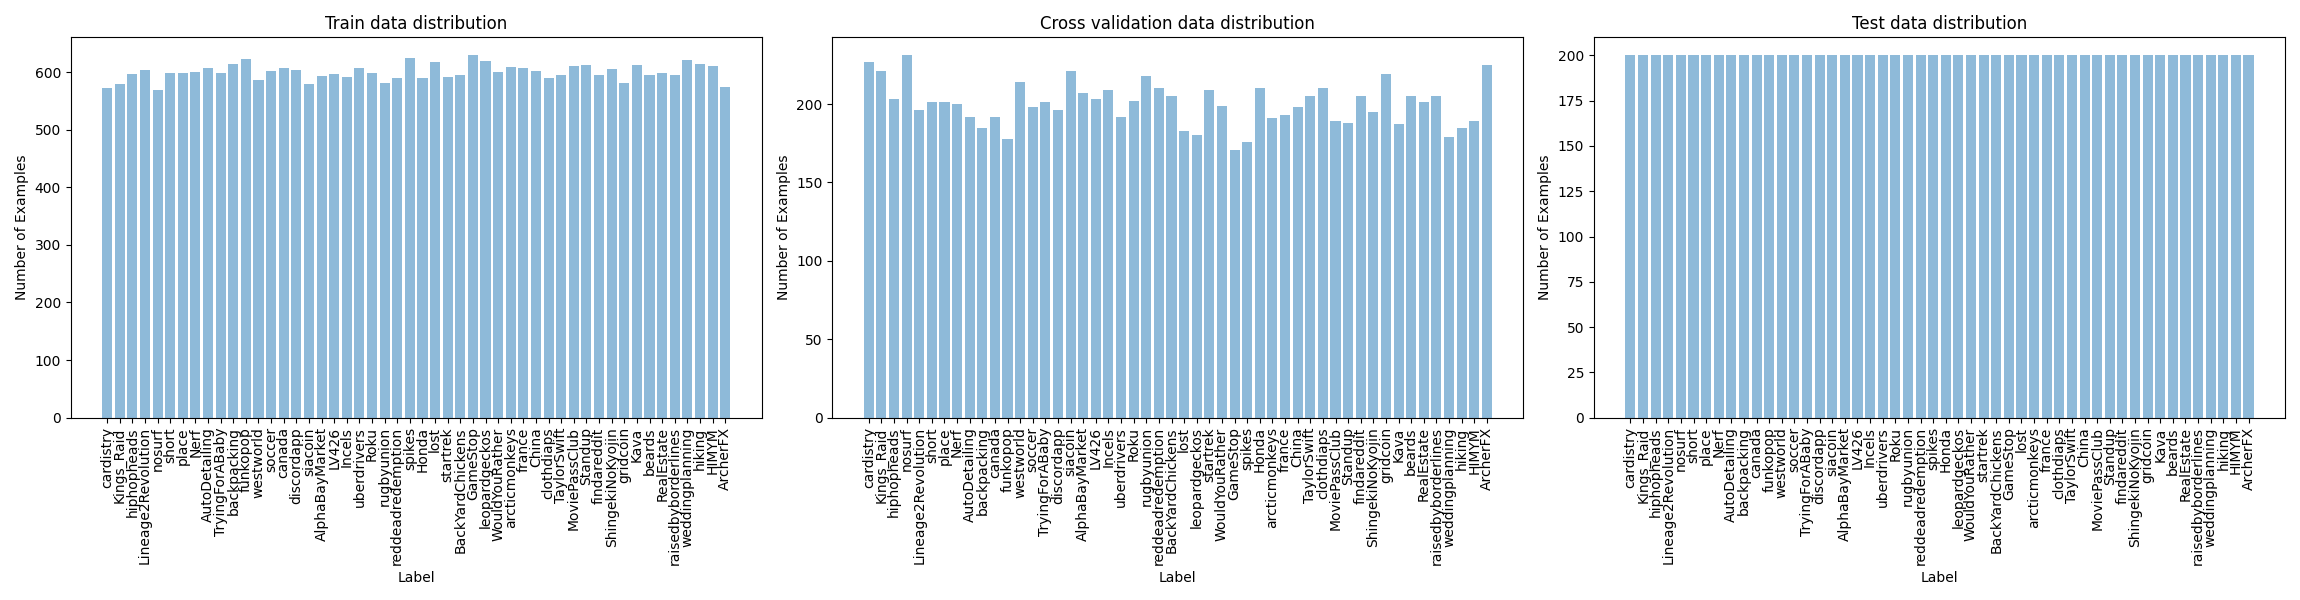
\includegraphics[width=\textwidth]{all_distribution_cv}
	\caption{Distribuição de dados por \textit{label} por \textit{dataset}, havendo discriminação entre dados de treino e de \textit{cross validation}.}
	\label{fig:data_distribution_with_cv}
\end{figure*}


\subsection{Resultados obtidos}
\label{sub:results_bayes}

Para obter os resultados que iremos descrever de seguida, adaptamos o código que encontramos no \textit{Kaggle} deste autor e fizemos algumas alterações de forma a usar a nossa técnica de extracção de \textit{features} dos dados, explicada na secção \ref{subsub:data_pre_processing}, ao invés da utilizada pelo autor. 

Desta forma, para 50 classes (ao invés das 5 usadas pelo autor original), obtivemos a variação de \textit{accuracy} de acordo com a variação do valor de alfa \footnote{\textit{Learning rate}} para os dados de treino e de \textit{cross validation} apresentados no gráfico da figura \ref{diagram:accuracy_alfa_bayes}. Como se pode verificar neste gráfico, foi obtido um valor máximo de $accuracy = 0.845$ para $\alpha = 0.1$ quando submetemos o modelo aos dados de \textit{cross validation}. 

\begin{figure}[t]
\begin{center}
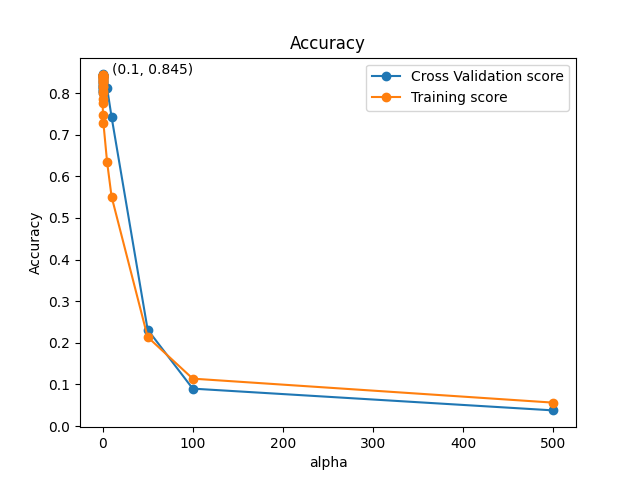
\includegraphics[width=0.5\textwidth,keepaspectratio]{figures/accuracy_alpha.png}
\caption{Gráfico da variação da \textit{accuracy} para valores de alfa entre $1*10^{-10}$ e $5*10^{2}$, para os dados de treino e de \textit{cross validation}}
\label{diagram:accuracy_alfa_bayes}
\centering
\end{center}
\end{figure}

O nosso passo seguinte foi retreinar o modelo onde obtivemos maior valor de alfa, usando como dados de treino os dados previamente usados para treino e \textit{cross validation}, ou seja, 80\% dos dados usados. Os resultados das métricas de performance por classe e totais quando o modelo foi treinado nas condições referidas podem ser consultados na tabela \ref{tab:bayes_perforamnce}. Duma forma geral, podemos verificar que temos resultados aceitáveis, mas não extraordinários (a \textit{accuracy} está longe de ser 100\%).

\begin{table}[!t]
\caption{Métricas de performance para $\alpha = 0.1$}
\begin{center}
\begin{tabular}{l c c c c}
Class & Accuracy & Recall & Precision & F1 Score\\ \hline
0 & 0.855 & 0.855 & 0.905 & 0.879\\
1 & 0.79 & 0.79 & 0.903 & 0.843\\
2 & 0.885 & 0.885 & 0.868 & 0.876\\
3 & 0.92 & 0.92 & 0.944 & 0.932\\
4 & 0.66 & 0.66 & 0.75 & 0.702\\
5 & 0.83 & 0.83 & 0.79 & 0.81\\
6 & 0.88 & 0.88 & 0.907 & 0.893\\
7 & 0.915 & 0.915 & 0.88 & 0.897\\
8 & 0.78 & 0.78 & 0.729 & 0.754\\
9 & 0.95 & 0.95 & 0.931 & 0.941\\
10 & 0.835 & 0.835 & 0.879 & 0.856\\
11 & 0.92 & 0.92 & 0.92 & 0.92\\
12 & 0.805 & 0.805 & 0.92 & 0.859\\
13 & 0.935 & 0.935 & 0.921 & 0.928\\
14 & 0.88 & 0.88 & 0.846 & 0.863\\
15 & 0.895 & 0.895 & 0.937 & 0.916\\
16 & 0.965 & 0.965 & 0.889 & 0.926\\
17 & 0.92 & 0.92 & 0.953 & 0.936\\
18 & 0.845 & 0.845 & 0.837 & 0.841\\
19 & 0.815 & 0.815 & 0.867 & 0.84\\
20 & 0.905 & 0.905 & 0.896 & 0.9\\
21 & 0.945 & 0.945 & 0.926 & 0.936\\
22 & 0.84 & 0.84 & 0.853 & 0.846\\
23 & 0.72 & 0.72 & 0.623 & 0.668\\
24 & 0.965 & 0.965 & 0.928 & 0.946\\
25 & 0.64 & 0.64 & 0.715 & 0.675\\
26 & 0.875 & 0.875 & 0.888 & 0.882\\
27 & 0.97 & 0.97 & 0.965 & 0.968\\
28 & 0.965 & 0.965 & 0.858 & 0.908\\
29 & 0.695 & 0.695 & 0.675 & 0.685\\
30 & 0.685 & 0.685 & 0.811 & 0.743\\
31 & 0.79 & 0.79 & 0.81 & 0.8\\
32 & 0.94 & 0.94 & 0.935 & 0.938\\
33 & 0.805 & 0.805 & 0.782 & 0.793\\
34 & 0.81 & 0.81 & 0.72 & 0.762\\
35 & 0.945 & 0.945 & 0.945 & 0.945\\
36 & 0.865 & 0.865 & 0.779 & 0.82\\
37 & 0.895 & 0.895 & 0.836 & 0.865\\
38 & 0.85 & 0.85 & 0.944 & 0.895\\
39 & 0.91 & 0.91 & 0.74 & 0.816\\
40 & 0.925 & 0.925 & 0.845 & 0.883\\
41 & 0.76 & 0.76 & 0.694 & 0.726\\
42 & 0.825 & 0.825 & 0.864 & 0.844\\
43 & 0.925 & 0.925 & 0.916 & 0.92\\
44 & 0.67 & 0.67 & 0.753 & 0.709\\
45 & 0.93 & 0.93 & 0.964 & 0.947\\
46 & 0.815 & 0.815 & 0.795 & 0.805\\
47 & 0.87 & 0.87 & 0.93 & 0.899\\
48 & 0.79 & 0.79 & 0.849 & 0.819\\
49 & 0.845 & 0.845 & 0.96 & 0.899\\
\hline
Macro Average & 0.853 & 0.853 & 0.856 & 0.853\\
\end{tabular}
\label{tab:bayes_perforamnce}
\end{center}
\end{table}


\subsection{Conclusão}

Apesar dos resultados finais obtidos terem sido aceitáveis, mas não extraordinários como demonstrado anteriormente, conseguimos obter um melhor valor de \textit{accuracy} que o autor da solução apresentada no inicio desta secção (aproximadamente $0.61$, para 5 classes, que ele obteve e $0.853$, para 50 classes, que nós obtivemos). Sendo que a maior alteração que fizemos à sua solução foi a utilização de um pré-processamento e selecção de \textit{features} distinta, concluímos que terá sido essa a chave para o nosso maior sucesso.

\section{Estudo com Regressão Logística}

A \textbf{Regressão Logística} é um algoritmo que permite, estatisticamente e a partir dum conjuntos de observações de eventos passados, criar um modelo que possibilite a previsão de valores associados a um possível evento (caracterizado por um conjunto de variáveis).

Apesar de termos encontrado o trabalho apresentado na secção \ref{sec:bayes}, encontra-mos também outros trabalhos que se insidiam na catalogação de texto, mas que não utilizavam o \textit{dataset} que usámos. Um destes trabalhos foi um criado por um outro utilizador do \textit{Kaggle}, em que usava, entre outros algoritmos, \textbf{Regressão Logística} para catalogar o tema de noticias da \textit{BBC}. O seu estudo pode ser encontrado em \cite{kaggle_logistic}. Neste estudo é notado que foi atingida uma \textit{accuracy} para os dados de teste de $0.79$ para as 20 classes em estudo.

\subsection{Repartição dos dados}
A divisão dos dados neste estudo foi a mesma usada descrita na secção \ref{subsub:bayes_data}.


\subsection{Resultados obtidos}

Tal como na secção \ref{sub:results_bayes}, começamos por adaptar o código do autor original. Neste caso, sendo que ele possuía vários algoritmos para realizar o seu estudo, foi necessário filtrar só o código correspondente ao estudo de \textit{Regressão Logística}. Tal como no estudo das Redes de Bayes, neste caso usamos também a técnica de extracção de \textit{features} explicada na secção \ref{subsub:data_pre_processing} ao invés da usada pelo autor.

Ao fazermos o estudo da variação do hiperparâmetro C \footnote{Parâmetro de regularização. Quanto maior o seu valor, maior será a \textit{regularization strength}}, para 5000 iterações com \textit{early stopping}, obtivemos a variação de \textit{accuracy} apresentada no gráfico da figura \ref{diagram:accuracy_c_logistic}. Com este gráfico pode-se concluir que o maior valor da \textit{accuracy} para os dados de \textit{cross validation} foi obtido para um valor de $C = 10^{4}$.

\begin{figure}[t]
\begin{center}
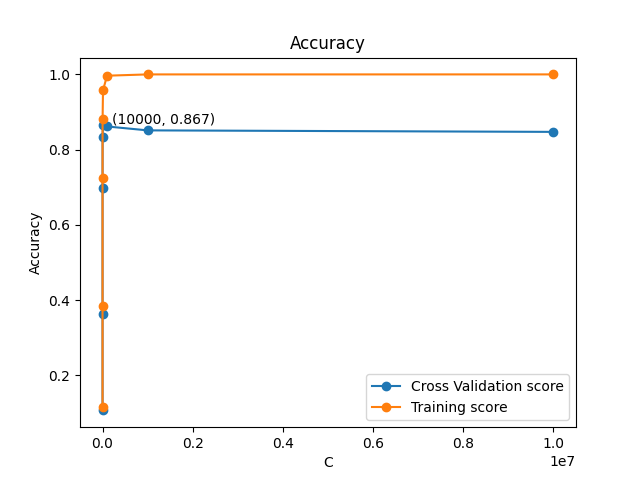
\includegraphics[width=0.5\textwidth,keepaspectratio]{figures/accuracy_C.png}
\caption{Gráfico da variação da \textit{accuracy} para valores de C entre $10^{0}$ e $10^{7}$, para os dados de treino e de \textit{cross validation}}
\label{diagram:accuracy_c_logistic}
\centering
\end{center}
\end{figure}

Desta forma, o nosso passo seguinte foi retreinar o melhor modelo obtido ($C = 10^{4}$) com os dados usados previamente para treino e \textit{cross validation}. As métricas de performance obtidas quando submetido o modelo final aos dados de teste podem ser consultadas na tabela \ref{tab:logistic_perforamnce}.

\begin{table}[!t]
\caption{Métricas de performance para $C = 10^{4}$}
\begin{center}
\begin{tabular}{l c c c c}
Class & Accuracy & Recall & Precision & F1 Score\\ \hline
0 & 0.9 & 0.9 & 0.893 & 0.998\\
1 & 0.805 & 0.805 & 0.957 & 0.895\\
2 & 0.85 & 0.85 & 0.949 & 0.902\\
3 & 0.9 & 0.9 & 0.965 & 0.954\\
4 & 0.795 & 0.795 & 0.909 & 0.858\\
5 & 0.91 & 0.91 & 0.917 & 0.92\\
6 & 0.895 & 0.895 & 0.986 & 0.929\\
7 & 0.91 & 0.91 & 0.964 & 0.993\\
8 & 0.815 & 0.815 & 0.868 & 0.829\\
9 & 0.95 & 0.95 & 0.996 & 0.983\\
10 & 0.785 & 0.785 & 0.943 & 0.901\\
11 & 0.935 & 0.935 & 0.985 & 0.976\\
12 & 0.815 & 0.815 & 0.925 & 0.997\\
13 & 0.94 & 0.94 & 0.985 & 0.961\\
14 & 0.835 & 0.835 & 0.85 & 0.879\\
15 & 0.865 & 0.865 & 0.957 & 0.943\\
16 & 0.96 & 0.96 & 0.988 & 0.992\\
17 & 0.91 & 0.91 & 0.987 & 0.991\\
18 & 0.855 & 0.855 & 0.991 & 0.891\\
19 & 0.875 & 0.875 & 0.967 & 0.911\\
20 & 0.895 & 0.895 & 0.955 & 0.897\\
21 & 0.96 & 0.96 & 0.944 & 0.941\\
22 & 0.845 & 0.845 & 0.8 & 0.947\\
23 & 0.775 & 0.775 & 0.928 & 0.764\\
24 & 0.955 & 0.955 & 0.992 & 0.999\\
25 & 0.73 & 0.73 & 0.896 & 0.885\\
26 & 0.87 & 0.87 & 0.911 & 0.925\\
27 & 0.96 & 0.96 & 0.995 & 0.983\\
28 & 0.935 & 0.935 & 0.897 & 0.968\\
29 & 0.845 & 0.845 & 0.868 & 0.942\\
30 & 0.82 & 0.82 & 0.983 & 0.969\\
31 & 0.875 & 0.875 & 0.933 & 0.889\\
32 & 0.91 & 0.91 & 0.98 & 0.983\\
33 & 0.84 & 0.84 & 0.92 & 0.972\\
34 & 0.85 & 0.85 & 0.946 & 0.837\\
35 & 0.955 & 0.955 & 0.981 & 0.986\\
36 & 0.905 & 0.905 & 0.872 & 0.87\\
37 & 0.89 & 0.89 & 0.918 & 0.987\\
38 & 0.87 & 0.87 & 0.954 & 0.884\\
39 & 0.89 & 0.89 & 0.92 & 0.998\\
40 & 0.905 & 0.905 & 0.896 & 0.921\\
41 & 0.745 & 0.745 & 0.892 & 0.837\\
42 & 0.835 & 0.835 & 0.98 & 0.896\\
43 & 0.9 & 0.9 & 0.977 & 0.949\\
44 & 0.88 & 0.88 & 0.986 & 0.899\\
45 & 0.945 & 0.945 & 0.989 & 0.964\\
46 & 0.835 & 0.835 & 0.974 & 0.957\\
47 & 0.915 & 0.915 & 0.959 & 0.941\\
48 & 0.865 & 0.865 & 0.932 & 0.984\\
49 & 0.905 & 0.905 & 0.985 & 0.978\\
\hline
Macro Average & 0.876 & 0.876 & 0.943 & 0.933\\
\end{tabular}
\label{tab:logistic_perforamnce}
\end{center}
\end{table}


\subsection{Conclusão}
Tal como na secção \ref{sec:bayes}, conseguimos neste exemplo obter uma performance melhor que a do autor do estudo original. Enquanto que este obteu uma \textit{accuracy} de teste de aproximadamente $0.79$ para apenas 20 classes, nós conseguimos obter uma \textit{accuracy} de aproximadamente $0.876$.

\section{Conclusões}
Finalizado este estudo, foi nos possível consolidar o nosso conhecimento relativamente aos algoritmos mais populares usados em \textit{Machine learning}, mais especificamente em processos de classificação multi-classe. 

O foco deste trabalho foi fazer a classificação de textos de \textit{posts} da plataforma \textit{Reddit}. Inicialmente pensávamos que a iniciação deste trabalho fosse mais fácil na medida em que este se trata de um problema de \textit{text classification} e existe muita informação relativa a este tópico. Após algumas tentativas de aplicar os algoritmos mais genéricos de \textit{text classification}, apercebemos-nos que estes não tinham uma boa performance, justificável pela imprevisibilidade dos textos no que toca à formalidade, o que torna a obtenção de \textit{features} mais difícil.

Numa fase inicial o esforço foi todo focado na etapa de pré-processamento dos textos, pois esta é bastante importante para a performance geral do modelo. Nesta etapa é feita a transformação de texto no formato \textit{"raw"} em vectores numéricos capazes de transmitir informações sobre os textos. Num problema deste tipo, a dimensão das \textit{features} de entrada é igual ao tamanho do vocabulário definido para o \textit{corpus} em questão. Logo, devido a isto, foi necessário fazer a segmentação do vocabulário original, pois este atinge dimensões nas ordens dos milhões, o que acaba por ser um número elevado de \textit{features} de entrada do modelo.


Foi possível concluir que especificamente para este \textit{dataset}, o algoritmo que obteve melhor performance foi o de \textit{Logistic Regression}. Contudo, é de ter em atenção que o treino de modelos que usem este algoritmo para uma grande quantidade de \textit{features} e de dados de treino se torna penosamente lento. Por exemplo, para o melhor modelo que obtivemos, o modelo demorou aproximadamente 4 horas a ser treinado, o que em algumas implementações pode não ser o mais aceitável. Sendo assim, os modelos de redes neuronais e de redes de \textit{bayes} apresentados, apesar de não terem tido uma prestação tão boa, podem ter uma utilização mais aceitável em circunstâncias em que o tempo de treino tenha de ser reduzido (estes dois modelos demoraram entre 2 a 3 minutos a serem treinados).

Neste trabalho reforçou-se ainda mais a ideia que a performance de um modelo de \textit{machine learning} está muito relacionada com a qualidade e processamento do \textit{dataset}, daí que muita das vezes um esforço inicial seja para regularizar e optimizar o conteúdo do \textit{dataset}, de forma a que o modelo consiga tirar partido da qualidade de selecção de \textit{features} e ecossistema do \textit{dataset}. Este facto provou-se na prática neste trabalho quando, se compara o uso de dois algoritmos (redes de \textit{bayes} deste relatório e rede de bayes de um \textit{paper}) iguais com processamentos de dados diferentes, o esforço colocado nesse aspecto neste trabalho trouxe benefícios na performance geral do modelo.

\section{Agradecimentos}
Queremos aqui deixar um agradecimento especial ao doutor engenheiro Mário Antunes do Instituto de Telecomunicações, que se demonstrou sempre disponível para esclarecer algumas dúvidas que fomos colocando e fez questão de acompanhar a evolução do nosso projecto.


\bibliographystyle{IEEEtran}
\bibliography{bibliography.bib}

\end{document}
